\chapter{Symulacyjna weryfikacja tezy}

Weryfikacja przedstawionego w pracy modelu błędu i wynikających z niego założeń odbędzie się w pierwszej kolejności metodą symulacyjną. W bieżącym rozdziale przedstawiony zostanie przykładowy tor pomiarowy, a następnie zostaną w nim wyróżnione kolejne źródła błędów. Na podstawie przedstawionego wcześniej modelu błędu opisane zostaną związki zachodzące pomiędzy błędami i oszacowana zostanie niepewność wielkości wyjściowych analizowanego toru pomiarowego. Wyniki uzyskane za pomocą zaproponowanego modelu zostaną porównane z wynikami uzyskanymi metodą Monte-Carlo. Omawiana analiza zostanie przeprowadzona z osobna dla każdego fragmentu toru pomiarowego, a następnie na podstawie ustalonych związków między błędami oszacowana zostanie niepewność rozszerzona wielkości wyjściowych analizowanego toru pomiarowego.

Przykładowy tor pomiarowy składać się będzie z przetwornika pomiarowego, który przekształcać będzie ciągłą w czasie wielkość fizyczną $s(t)$ na reprezentujący ją sygnał napięciowy $y_{a}(t)$. Sygnał wyjściowy przetwornika pomiarowego poddawany będzie wzmocnieniu w celu dopasowania jego poziomu do zakresu napięcia wejściowego przetwornika analogowo-cyfrowego. Wzmocniony sygnał $y_{b}(t)$ podawany będzie na wejście przetwornika analogowo-cyfrowego, którego wielkości wyjściowe oznaczono symbolem $x_{c}(i)$. Ostatecznie sygnał wyjściowy przetwornika analogowo-cyfrowego trafiać będzie na wejście algorytmu dyskretnej transformacji falkowej, a na jego podstawie wyznaczany będzie wektor wielkości wyjściowych oznaczonych jako $X(k)$. Schemat ideowy opisanego toru pomiarowego przedstawiono na rysunku~\ref{fig:chain_symul}.

\begin{figure}[htb!]
\begin{center}
\includegraphics{obrazki/schemat_symul}
\makecaption{fig:chain_symul}{Schemat blokowy toru pomiarowego będącego obiektem przeprowadzanego eksperymentu symulacyjnego}
\end{center}
\end{figure}

Podczas eksperymentu przyjmuje się, że przetwarzany sygnał pomiarowy będzie obarczony błędem związanym z szumem, o stałej widmowej gęstości mocy i rozkładzie normalnym. Przetwornik pomiarowy, zastosowany w celu przetworzenia analizowanego sygnału wejściowego na postać napięciową, posiadać będzie pewną częstotliwość graniczną, a jego charakterystyka nie będzie idealnie liniowa. Zastosowany wzmacniacz pomiarowy również cechować się będzie pewną częstotliwością graniczną, natomiast zakłada się, że nieliniowość jego charakterystyki będzie pomijalnie mała. Temperatura otoczenia wpływać będzie na dryf zera przetwornika pomiarowego oraz wzmacniacza, przy czym temperatura ta nie będzie mierzona, zatem jej wpływ na wyniki pomiaru nie będzie korygowany. Zastosowany przetwornik analogowo-cyfrowy wprowadzać będzie błąd związany z kwantowaniem przetwarzanej wielkości. Algorytm transformacji falkowej wprowadzać będzie do wielkości wyjściowych błąd własny związany z zaokrągleniami.

W dalszej części rozdziału omówione zostaną kolejne elementy toru pomiarowego, ich wpływ na przetwarzany sygnał oraz relacje pomiędzy błędami na wejściu i wyjściu tych fragmentów. Przedstawione zostaną również szczegółowe założenia odnośnie właściwości opisanych we wprowadzeniu fragmentów toru pomiarowego. Dla przeprowadzonego eksperymentu przyjmuje się, że przetwarzany sygnał $s(t)$ określony jest w postaci:
\begin{gather}
\dot{s} \emb{t} = \frac{6}{10} \sin \left( 2 \pi f_{1} t \right) - \frac{3}{10} \sin \left( 10 \pi f_{1} t + \frac{\pi}{8} \right) + \frac{1}{10} \sin \left( 30 \pi f_{1} t + \frac{\pi}{6} \right) \label{eq:sym_in_ideal}, \\
\tilde{s} \emb{t} = \dot{s} \emb{t} + e_{s,r} \emb{t} \label{eq:sym_in_real},
\end{gather}
przy czym $f_{1} = \qty{1}{kHz}$, natomiast $\sigma_{s,r}^{2} = \frac{2}{3} \cdot 10^{-5}$. Parametry kolejnych harmonicznych przetwarzanego sygnału zostały zestawione w tabeli~\ref{tab:sym_in_params_ideal}. Przetwarzany sygnał będzie próbkowany ze stałą częstotliwością $f_{s} = \qty{48}{kHz}$. Do wyznaczenia wektora wielkości wyjściowych algorytmu dyskretnej transformacji falkowej koniecznych będzie $N = 8$ próbek wielkości wejściowych tego algorytmu, na podstawie których wyznaczonych zostanie $M = 8$ próbek wielkości wyjściowych toru pomiarowego.

\begin{table}[htb!]
\begin{center}
\makecaption{tab:sym_in_params_ideal}{Parametry kolejnych harmonicznych przetwarzanego sygnału niezakłóconego błędami przyjęte w przeprowadzanym eksperymencie symulacyjnym}
\begin{tabular}[c]{| c | c | S[table-format = +1.1] | c |} \hline
\textbf{Lp. $i$} & \textbf{Pulsacja $\omega_{s,i}$, rad/s} & \textbf{Amplituda $E_{s,o}(\omega_{s,i})$} & \textbf{Faza $\varphi_{s,o}(\omega_{s,i})$, rad} \\ \hline
1 & $1000  \cdot 2\pi$ &  0.6 & $0$       \\ \hline
2 & $5000  \cdot 2\pi$ & -0.3 & $\pi / 8$ \\ \hline
3 & $15000 \cdot 2\pi$ &  0.1 & $\pi / 6$ \\ \hline
\end{tabular}
\end{center}
\end{table}

Eksperyment zakłada, że okres próbkowania będzie stały dla każdej próbki przetwarzanego sygnału, natomiast okno pomiarowe będzie usytuowane losowo względem przebiegu przetwarzanego sygnału. Dodatkowo wprowadza się założenie, że temperatura otoczenia przyjmować może dowolną wartość z zakresu $<17;23>\unit{\degreeCelsius}$, przy czym wartością oczekiwaną temperatury jest wartość \qty{20}{\degreeCelsius}, a w obrębie wskazanego przedziału rozkład wartości temperatury jest rozkładem trójkątnym. Ze względu na dużą inercję, przyjmuje się że zmiany temperatury w czasie wykonywania serii pomiarów potrzebnych do wyznaczenia wektora wielkości wyjściowych toru pomiarowego będą bardzo niewielkie, a zatem błędy związane z dryfem temperaturowym rozpatrywane będą w kategorii błędów statycznych.

\section{Analiza przetwornika pomiarowego}

Zastosowany w przykładzie przetwornik pomiarowy przekształca sygnał $s(t)$, związany z mierzoną wielkością fizyczną, na wyjściowy sygnał napięciowy $y_{a}(t)$. Przyjmuje się, że wielkość fizyczna zmieniać się może w zakresie $<0;1>$, przy czym czułość przetwornika pomiarowego będzie równa jedności, a jego częstotliwość graniczna wyniesie $f_{a,g} = \qty{320}{kHz}$. Wobec powyższych, wartość wielkości wyjściowej $y_{a}(t)$ mieścić się będzie w przedziale $<0;1>\unit{V}$. Charakterystyka omawianego obiektu jest zależna od temperatury otoczenia, przy czym temperatura ta nie jest mierzona w trakcie wykonywania pomiarów. Stosując zaproponowany w pracy model błędu, opisać można przebieg wielkości wyjściowej analizowanego obiektu na podstawie równań od~\eqref{eq:out_cont_ideal_all} do~\eqref{eq:out_cont_err_sum_all}, które w przedstawionym przypadku przyjmują postać:
\begin{gather}
\dot{y}_{a} \emb{t} = \dot{s} \emb{t} \label{eq:sym_parta_out_ideal}, \\
\tilde{y}_{a} \emb{t} = \dot{y}_{a} \emb{t} + e_{a,\Sigma} \emb{t} \label{eq:sym_parta_out_real},
\end{gather}
przy czym błędy cząstkowe zawarte w błędzie wypadkowym $e_{a,\Sigma}$ zostaną omówione w dalszej cześć podrozdziału.

Opisywane w założeniach eksperymentu zmiany temperatury otoczenia będą bardzo niewielkie w obrębie pojedynczej serii pomiarowej. Można zatem przyjąć, że błąd wynikający z wpływu temperatury na wartość wielkości wyjściowej analizowanego obiektu będzie stały w obrębie okna pomiarowego, a zatem kwalifikowany on będzie jako błąd statyczny. W eksperymencie zakłada się, że dryf temperaturowy związany z błędem statycznym własnym jest określony następującym równaniem:
\begin{equation}
e_{a,sw} \emb{t} = f_{a,z} \left( \vartheta \emb{t} \right) = \frac{3}{2} \left( \vartheta \emb{t} - \qty{20}{\degreeCelsius} \right) ~\unit{\frac{mV}{K}} \label{eq:sym_parta_stat_err},
\end{equation}
gdzie $\vartheta$ jest rzeczywistą temperaturą otoczenia wyrażoną w stopniach Celsjusza. Można zatem określić wariancję oraz niepewność rozszerzoną omawianego błędu zależnościami:
\begin{gather}
\sigma_{a,sw}^{2} = \frac{\left( -\frac{9}{2} 10^{-3} \right)^{2} + \left( \frac{9}{2} 10^{-3} \right)^{2} - \left( -\frac{9}{2} 10^{-3} \right) \left( \frac{9}{2} 10^{-3} \right)}{18} = 3 \frac{3}{8} ~\unit{\micro V} \label{eq:sym_parta_stat_var}, \\
U_{a,sw} = c_{t} \sigma_{a,rw} = \frac{5.7 \sqrt{6}}{4} ~\unit{mV} \label{eq:sym_parta_stat_unc},
\end{gather}
gdzie $c_{t}$ jest współczynnikiem rozszerzenia dla rozkładu trójkątnego i przy poziomie ufności $\alpha = 95\%$ wynosi $1.90$.

Funkcja przetwarzania obiektu, wynikająca z przedstawionych we wstępie do podrozdziału założeń, powinna być określona równaniem liniowym w postaci:
\begin{equation}
\dot{f}_{a} \emb{x} = x \label{eq:sym_parta_statfun},
\end{equation}
natomiast przyjmuje się, że rzeczywista funkcja przetwarzania $\tilde{f}_{a}(x)$, uwzględniająca nieliniowość zastosowanego przetwornika, nie jest znana. Zakłada się jednak, że błąd wynikający z nieliniowości charakterystyki przyjmuje wartość z przedziału $<-\sqrt{10};\sqrt{10}>\unit{mV}$, a dodatkowo uzyskanie każdej z wartości jest jednakowo prawdopodobne. Wobec powyższych, jeżeli pomiar będzie przeprowadzany wielokrotnie, można rozważany błąd opisywać w kategoriach probabilistycznych, wliczając jego udział do puli błędów losowych. Wariancję oraz niepewność rozszerzoną, związane z omawianym błędem losowym własnym $e_{a,rw}(t)$, wyrazić można w postaci:
\begin{gather}
\sigma_{a,rw}^{2} = \frac{\left( \left( \sqrt{10} \cdot 10^{-3} \right) + \left( \sqrt{10} \cdot 10^{-3} \right) \right)^{2}}{12} = 3 \frac{1}{3} ~\unit{\micro V} \label{eq:sym_parta_rand_self_var}, \\
U_{a,rw} = c_{u} \sigma_{a,rw} = \frac{1.65 \sqrt{30}}{3} ~\unit{mV} \label{eq:sym_parta_rand_self_unc},
\end{gather}
przy czym $c_{u}$ jest współczynnikiem rozszerzenia dla rozkładu jednostajnego i przy poziomie ufności $\alpha = 95\%$ wynosi $1.65$ \cite{jcgm_guide}.

Kolejną grupą właściwości obiektu są właściwości dynamiczne, związane z jego częstotliwością graniczną. Przypadek idealny zakłada, że analizowany obiekt nie powinien mieć żadnego wpływu na widmo przetwarzanego sygnału, a zatem transmitancja tego obiektu powinna wynosić $\dot{G}_{a}(j\omega) = 1$. Na podstawie założonych parametrów rzeczywistych obiektu przyjmuje się, że transmitancja $\tilde{G}_{a}(j\omega)$ wynosi:
\begin{equation}
\tilde{G}_{a} \emb{j\omega} = \frac{1}{1 + j \frac{\omega}{2 \pi f_{a,g}}} = \frac{1}{\frac{\omega^{2}}{4 \pi^{2} f_{a,g}^{2}} + 1} - j \frac{\omega}{2 \pi f_{a,g} \left( \frac{\omega^{2}}{4 \pi^{2} f_{a,g}^{2}} + 1 \right) } \label{eq:sym_parta_trans},
\end{equation}
a zatem równania~\eqref{eq:mid_cont_amp} oraz~\eqref{eq:mid_cont_phi} przyjmują w tym przypadku postać:
\begin{gather}
\tilde{K}_{a} \emb{\omega} = \left( \frac{\omega^{2}}{4 \pi^{2} f_{a,g}^{2}} + 1 \right)^{-\frac{1}{2}} \label{eq:sym_parta_amp_real}, \\
\tilde{\varphi}_{a} \emb{\omega} = \arctan \left( -\frac{\omega}{2 \pi f_{a,g}} \right) \label{eq:sym_parta_phi_real},
\end{gather}
przy czym dla idealnej transmitancji $\dot{G}_{a}(j\omega)$ parametry te wynoszą kolejno:
\begin{gather}
\dot{K}_{a} \emb{\omega} = 1 \label{eq:sym_parta_amp_ideal}, \\
\dot{\varphi}_{a} \emb{\omega} = 0 \label{eq:sym_parta_phi_ideal},
\end{gather}
co oznacza, że w sytuacji idealnej wzmocnienie układu jest niezależnie od częstotliwości sygnału i równe jedności oraz że obiekt ten nie wprowadza żadnego przesunięcia w fazie przetwarzanego sygnału -- co odbiega od analizowanej sytuacji rzeczywistej.

Przedstawione zależności oraz zaproponowana w równaniu~\eqref{eq:mid_cont_var_rand} metoda pozwalają oszacować średnią wariancję błędu związanego z szumem zawartym w przetwarzanej wielkości wejściowej w zakresie częstotliwości od $<0;f_{p}>$ oraz związaną z nią niepewność rozszerzoną w postaci:
\begin{gather}
\sigma_{a,rp}^{2} = \frac{1}{\omega_{p}} \int _{0} ^{\omega_{p}} \tilde{K}_{a}^{2} \emb{\omega} \sigma_{s,r}^{2} d\omega = \sigma_{s,r}^{2} = 6 \frac{2}{3} ~\unit{\micro V} \label{eq:sym_parta_rand_prop_var}, \\
U_{a,rp} = c_{u} \sigma_{a,rp} = \frac{3.92 \sqrt{15}}{3} ~\unit{mV} \label{eq:sym_parta_rand_prop_unc},
\end{gather}
gdzie $\omega_{p} = 2 \pi f_{p}$ jest pulsacją próbkowania. Zauważyć można, że w analizowanym zakresie częstotliwości wartość wzmocnienia $\tilde{K}_{a}(\omega)$ jest zbliżona do jedności, a zatem transmitancja obiektu nie wpływa na widmo przetwarzanego szumu. Można zatem uznać, że wariancja błędu losowego propagowanego na wyjściu jest identyczna, jak na wejściu obiektu.

Na podstawie równania~\eqref{eq:mid_cont_err_dyn_self}, błąd własny dynamiczny w funkcji częstotliwości wybranej harmonicznej sygnału opisać można następującą zależnością:
\begin{equation}
\begin{split}
e_{a,dw} \emb{t,\omega} = ~
& \tilde{K}_{a} \emb{\omega} E_{s,o} \emb{\omega} \sin \left( \omega t + \varphi_{s,o} \emb{\omega} + \tilde{\varphi}_{a} \emb{\omega} \right) - \\
& \dot{K}_{a} \emb{\omega} E_{s,o} \emb{\omega} \sin \left( \omega t + \varphi_{s,o} \emb{\omega} + \dot{\varphi}_{a} \emb{\omega} \right)
\end{split}
\label{eq:sym_parta_dyn_self_err}.
\end{equation}
Jako, że sygnał wejściowy analizowanego obiektu nie jest obarczony błędem dynamicznym, nie ma potrzeby wykonywania analizy dla błędu dynamicznego propagowanego. Ze względu na fakt, że przedstawione przebiegi składowych harmonicznych błędu dynamicznego będą w kolejnych fragmentach toru pomiarowego przetwarzane ponownie, nie należy w tym miejscu wyznaczać wariancji całkowitego błędu dynamicznego. Aby umożliwić analizę propagacji błędów dynamicznych przez kolejne fragmenty toru pomiarowego, minimalizując jednocześnie liczbę analizowanych składowych błędu dynamicznego, wyznaczone zostaną na podstawie równań~\eqref{eq:dyn_vect_amp} oraz~\eqref{eq:dyn_vect_phi} wypadkowe parametry składowych błędu dla kolejnych harmonicznych. Należy zauważyć, że relacje pomiędzy amplitudą, a odchyleniem standardowym analizowanej harmonicznej opisuje równanie~\eqref{eq:dyn_std}. Analizując równanie~\eqref{eq:sym_parta_dyn_self_err} można zauważyć, że dla każdej harmonicznej błąd ten ma dwie składowe o przeciwnych znakach. Korzystając z właściwości funkcji \enquote{sinus} można odwrócić znak wybranej składowej oraz dodać kąt $\pi~\unit{rad}$ do argumentu tej funkcji, zachowując przy tym oryginalną wartość tej składowej. Przebieg składowej błędu dynamicznego własnego o częstotliwości \qty{1}{kHz} przedstawia następujące równanie:
\begin{equation}
\begin{split}
e_{a,dw} \emb{t,\omega} \left|_{\omega = 1000 \cdot 2 \pi } \right. = ~
& \tilde{K}_{a} \emb{\omega} E_{s,o} \emb{\omega} \sin \left( \omega t + \varphi_{s,o} \emb{\omega} + \tilde{\varphi}_{a} \emb{\omega} \right) - \\
& \dot{K}_{a} \emb{\omega} E_{s,o} \emb{\omega} \sin \left( \omega t + \varphi_{s,o} \emb{\omega} + \dot{\varphi}_{a} \emb{\omega} \right) = \\
& 1.0 \cdot 0.6 \cdot \sin \left( \omega t + 0 - \num{3.13e-3} \right) + \\
& 1.0 \cdot 0.6 \cdot \sin \left( \omega t + 0 + 0 + \pi \right)
\end{split}
\label{eq:sym_parta_dyn_self_example_harm}.
\end{equation}
Kolejne składowe dla wymienionych wcześniej harmonicznych sygnału błędu dynamicznego przedstawiono w tabeli~\ref{tab:sym_parta_params_dyn_list}, przy czym przedstawione wartości amplitudy i fazy wyznaczono przekształcając równanie~\eqref{eq:sym_parta_dyn_self_err} w sposób analogiczny, jak w przypadku równania~\eqref{eq:sym_parta_dyn_self_example_harm}.

\begin{table}[htb!]
\begin{center}
\makecaption{tab:sym_parta_params_dyn_list}{Parametry kolejnych harmonicznych błędu dynamicznego własnego analizowanego w eksperymencie symulacyjnym przetwornika pomiarowego}
\begin{tabular}[c]{| c | c | c | c |} \hline
\textbf{Lp. $i$} & \textbf{Pulsacja $\omega_{a,i}$, rad/s} & \textbf{Amplituda $E_{a,e}(\omega_{a,i})$, V} & \textbf{Faza $\varphi_{a,e}(\omega_{a,i})$, rad} \\ \hline
1 & \multirow{2}{*}{$1000  \cdot 2\pi$} &  $1.0 \cdot 0.6$       & $0 - \num{3.13e-3}$            \\ \cline{1-1} \cline{3-4}
2 &                                     &  $1.0 \cdot 0.6$       & $0 + 0 + \pi$                  \\ \hline
3 & \multirow{2}{*}{$5000  \cdot 2\pi$} &  $1.0 \cdot 0.3$       & $\pi/8 - \num{1.56e-2} + \pi$  \\ \cline{1-1} \cline{3-4}
4 &                                     &  $1.0 \cdot 0.3$       & $\pi/8 + 0$                    \\ \hline
5 & \multirow{2}{*}{$15000 \cdot 2\pi$} &  $1.0 \cdot 0.1$       & $\pi/6 - \num{4.69e-2}$        \\ \cline{1-1} \cline{3-4}
6 &                                     &  $1.0 \cdot 0.1$       & $\pi/6 + 0 +\pi$               \\ \hline
\end{tabular}
\end{center}
\end{table}

Przedstawiając składowe równania~\eqref{eq:sym_parta_dyn_self_example_harm} za pomocą wektorów, zgodnie z równaniem~\eqref{eq:dyn_vect}, a następnie sumując opisane składniki zgodnie z równaniem~\eqref{eq:dyn_vect_sum}, wyznaczyć można parametry błędu wypadkowego opisane równaniami~\eqref{eq:dyn_vect_amp} oraz~\eqref{eq:dyn_vect_phi}, przy czym w rozpatrywanym przypadku przyjmują one postać:
\begin{gather}
\mathbf{e}_{\Sigma,1} =
\begin{bmatrix}
0.6 \cos \emb{\num{-3.13e-3}} + 0.6 \cos \emb{\pi} & 0.6 \sin \emb{\num{-3.13e-3}} + 0.6 \sin \emb{\pi}
\end{bmatrix}
\label{eq:sym_parta_dyn_self_example_sum}, \\
E_{\Sigma,1} = \sqrt{\emb{\num{-5.86e-6}}^{2} + \emb{\num{-1.88e-3}}^{2}} = \qty{1.88}{mV} \label{eq:sym_parta_dyn_self_example_amp}, \\
\varphi_{\Sigma,1} = \arctan \emb{\frac{\num{-1.88e-3}}{\num{-5.86e-6}}} = \qty{-1.57}{rad} \label{eq:sym_parta_dyn_self_example_phi}.
\end{gather}
Dla pozostałych harmonicznych należy opisane powyżej wartości wyznaczyć w sposób analogiczny, przy czym omawiane wyniki zestawiono w tabeli~\ref{tab:sym_parta_params_dyn_summary}. Przedstawione wartości umożliwiają wyznaczenie na podstawie równania~\eqref{eq:dyn_std} odchylenia standardowego kolejnych składowych błędu oraz na podstawie równania~\eqref{eq:unc_sum} niepewności rozszerzonej, przy czym dla rozkładu dwumodalnego współczynnik rozszerzenia $c_{d}$ dla poziomu ufności $\alpha = 95\%$ wynosi $1.42$.

\begin{table}[htb!]
\begin{center}
\makecaption{tab:sym_parta_params_dyn_summary}{Parametry kolejnych harmonicznych błędu dynamicznego własnego analizowanego w eksperymencie symulacyjnym przetwornika pomiarowego}
\begin{tabular}[c]{| c | c | S[table-format = 1.2] | S[table-format = +1.2] |} \hline
\textbf{Lp. $j$} & \textbf{Pulsacja $\omega_{a,j}$, rad/s} & \textbf{Amplituda $E_{a,e}(\omega_{a,j})$, mV} & \textbf{Faza $\varphi_{a,e}(\omega_{a,j})$, rad} \\ \hline
1 & $1000  \cdot 2\pi$  &  1.88  & -1.57  \\ \hline
2 & $5000  \cdot 2\pi$  &  4.69  &  1.96  \\ \hline
3 & $15000 \cdot 2\pi$  &  4.68  & -1.07  \\ \hline
\end{tabular}
\end{center}
\end{table}

\begin{table}[htb!]
\begin{center}
\makecaption{tab:sym_parta_params_unc_list}{Budżet niepewności wielkości wyjściowej analizowanego w eksperymencie symulacyjnym przetwornika pomiarowego}
\begin{tabular}[c]{| c | c | S[table-format = 1.2] | S[table-format = 2.2] | c | c |} \hline
\textbf{Lp.} & \textbf{Symbol} & \textbf{$U_{95\%}$, mV} & \textbf{$\sigma^{2}$, \micro V} & \textbf{Rozkład} & \textbf{Źródło błędu} \\ \hline
1 & ${a,sw}$       & 3.49  &  3.38   & trójkątny                    & dryf temperatury                           \\ \hline
2 & ${a,rw}$       & 3.01  &  3.33   & jednostajny                  & nieliniowość obiektu                       \\ \hline
3 & ${a,rp}$       & 5.06  &  6.67   & normalny                     & szum wielkości wejściowej                  \\ \hline
4 & ${a,dw,1}$     & 1.87  &  1.77   & \multirow{3}{*}{dwumodalny}  & \multirow{3}{*}{transmitancja wzmacniacza} \\ \cline{1-4}
5 & ${a,dw,2}$     & 4.68  &  11.00  &                              &                                            \\ \cline{1-4}
6 & ${a,dw,3}$     & 4.67  &  10.95  &                              &                                            \\ \hline
\end{tabular}
\end{center}
\end{table}

Na podstawie przedstawionych dotychczas zależności określono budżet niepewności dla analizowanego fragmentu toru pomiarowego, który zestawiono w tabeli~\ref{tab:sym_parta_params_unc_list}. Należy zauważyć, że kolejne błędy cząstkowe w opisywanym przypadku nie są ze sobą skorelowane. Ostatnim krokiem analizy pozostaje zatem określenie wypadkowej wartości niepewności rozszerzonej dla analizowanego fragmentu toru pomiarowego. Na obecnym etapie analizy wyznaczanie niepewności wypadkowej nie jest konieczne i nie będzie wykorzystywane w dalszym procesie analizy -- przeprowadzenie tej operacji jest uzasadnione potrzebą weryfikacji skuteczności proponowanej metody. Zastosowane w obliczeniach współczynniki koherencji wyznaczono metodą Monte-Carlo, zgodnie z metodą opisaną w \cite{jakubiec_arithmetic, batko_uncertainty} na podstawie zależności~\eqref{eq:unc_coher}.

W pierwszej kolejności wyznaczone zostaną wypadkowe niepewności rozszerzone i wypadkowe wariancje z uwzględnieniem na wprowadzone kategorie błędów. W przypadku błędu statycznego, ze względu na istnienie tylko jednego źródła tego błędu, parametry wypadkowe będą identyczne, jak parametry błędu statycznego własnego. Można zatem zapisać, że:
\begin{gather}
U_{a,s} = U_{a,sw} = \qty{3.49}{mV} \label{eq:sym_parta_uncert_stat}, \\
\sigma_{a,s}^{2} = \sigma_{a,sw}^{2} = \qty{3.38}{\micro V} \label{eq:sym_parta_var_stat}.
\end{gather}
Dla błędów losowego i dynamicznego, wypadkowa niepewność rozszerzona wyznaczana jest zgodnie z zależnością~\eqref{eq:unc_matrix}, przy czym:
\begin{gather}
\begin{split}
U_{a,r} = ~
& \sqrt{
\begin{bmatrix}
U_{a,rw} \\ U_{a,rp}
\end{bmatrix}^{T}
\begin{bmatrix}
1           & h_{a,rw,rp} \\
h_{a,rw,rp} & 1
\end{bmatrix}
\begin{bmatrix}
U_{a,rw} \\ U_{a,rp}
\end{bmatrix}} = ~ \\
& \sqrt{
\begin{bmatrix}
3.01 \\ 5.06
\end{bmatrix}^{T}
\begin{bmatrix}
1.000 & 0.120 \\
0.120 & 1.000
\end{bmatrix}
\begin{bmatrix}
3.01 \\ 5.06
\end{bmatrix}} = \qty{6.19}{mV}
\end{split}
\label{eq:sym_parta_uncert_rand}, \\
\begin{split}
U_{a,d} = ~
& \sqrt{
\begin{bmatrix}
U_{a,dw,1} \\ U_{a,dw,2} \\ U_{a,dw,3}
\end{bmatrix}^{T}
\begin{bmatrix}
1            & h_{a,dw,1,2} & h_{a,dw,1,3} \\
h_{a,dw,2,1} & 1            & h_{a,dw,2,3} \\
h_{a,dw,3,1} & h_{a,dw,3,1} & 1                 \\
\end{bmatrix}
\begin{bmatrix}
U_{a,dw,1} \\ U_{a,dw,2} \\ U_{a,dw,3}
\end{bmatrix}} = ~ \\
& \sqrt{
\begin{bmatrix}
1.87 \\ 4.68 \\ 4.67
\end{bmatrix}^{T}
\begin{bmatrix}
1.000 & 0.359 & 0.358 \\
0.359 & 1.000 & 0.376 \\
0.358 & 0.376 & 1.000
\end{bmatrix}
\begin{bmatrix}
1.87 \\ 4.68 \\ 4.67
\end{bmatrix}} = \qty{8.73}{mV}
\end{split}
\label{eq:sym_parta_uncert_dyn}.
\end{gather}
Wypadkowa wariancja, ze względu na brak korelacji kolejnych źródeł błędów, wyznaczana jest zgodnie z zależnością~\eqref{eq:var_sum}, a zatem:
\begin{gather}
\sigma_{a,r}^{2} = \sigma_{a,rw}^{2} + \sigma_{a,rp}^{2} = \qty{10.00}{\micro V} \label{eq:sym_parta_var_rand}, \\
\sigma_{a,d}^{2} = \sigma_{a,dw,1}^{2} + \sigma_{a,dw,2}^{2} + \sigma_{a,dw,3}^{2} = \qty{23.72}{\micro V} \label{eq:sym_parta_var_dyn}.
\end{gather}
Dla przedstawionych sygnałów błędu oszacować można na podstawie równania~\eqref{eq:unc_sum} współczynniki rozszerzenia, przy czym:
\begin{gather}
c_{a,s} = c_{a,sw} = c_{t} = 1.90 \label{eq:sym_parta_factor_sta}, \\
c_{a,r} = \frac{U_{a,r}}{\sigma_{a,r}} = \frac{\qty{6.19}{mV}}{\qty{3.16}{mV}} = 1.96 \label{eq:sym_parta_factor_rand}, \\
c_{a,d} = \frac{U_{a,d}}{\sigma_{a,d}} = \frac{\qty{8.73}{mV}}{\qty{4.87}{mV}} = 1.79 \label{eq:sym_parta_factor_dyn}.
\end{gather}

Ostatnim krokiem analizy jest wyznaczenie wypadkowych parametrów wyjściowego sygnału błędu. Proces ten przeprowadzić można zarówno korzystając z opisanego tabelą~\ref{tab:sym_parta_params_unc_list} budżetu niepewności, jak i na podstawie parametrów wyznaczonych za pomocą równać od~\eqref{eq:sym_parta_uncert_stat} do~\eqref{eq:sym_parta_var_dyn}. W pierwszej kolejności przedstawiona zostanie metoda wykorzystująca budżet niepewności. Wypadkową niepewność rozszerzoną wyznaczyć można zapisując równanie~\eqref{eq:unc_matrix} w postaci:
\begin{equation}
U_{a,\Sigma} = \sqrt{\mathbf{U}_{a}^{T} \cdot \mathbf{h}_{a} \cdot \mathbf{U}_{a}} \label{eq:sym_parta_uncert_sum},
\end{equation}
gdzie wektor niepewności cząstkowych $\mathbf{U}_{a}$ przyjmuje postać:
\begin{equation}
\mathbf{U}_{a}^{T} =
\begin{bmatrix}
U_{a,sw} & U_{a,rw} & U_{a,rp} & U_{a,dw,1} & U_{a,dw,2} & U_{a,dw,3}
\end{bmatrix}
\label{eq:sym_parta_uncert_vector},
\end{equation}
natomiast macierz współczynników koherencji $\mathbf{h}_{a}$ opisana jest następująco:
\begin{equation}
\mathbf{h}_{a} =
\begin{bmatrix}
1             & h_{a,sw,rw}   & h_{a,sw,rp}   & h_{a,sw,dw,1} & h_{a,sw,dw,2} & h_{a,sw,dw,3} \\
h_{a,rw,sw}   & 1             & h_{a,rw,pw}   & h_{a,rw,dw,1} & h_{a,rw,dw,2} & h_{a,rw,dw,3} \\
h_{a,rp,sw}   & h_{a,rp,rw}   & 1             & h_{a,rp,dw,1} & h_{a,rp,dw,2} & h_{a,rp,dw,3} \\
h_{a,dw,1,sw} & h_{a,dw,1,rw} & h_{a,dw,1,rp} & 1             & h_{a,dw,1,2}  & h_{a,dw,1,3}  \\
h_{a,dw,2,sw} & h_{a,dw,2,rw} & h_{a,dw,2,rp} & h_{a,dw,2,1}  & 1             & h_{a,dw,2,3}  \\
h_{a,dw,3,sw} & h_{a,dw,3,rw} & h_{a,dw,3,rp} & h_{a,dw,3,1}  & h_{a,dw,3,2}  & 1             \\
\end{bmatrix}
\label{eq:sym_parta_uncert_coher},
\end{equation}
przy czym przykładowo, dla pary błędów statycznego własnego oraz losowego własnego, wartość współczynnika koherencji jest obliczana zgodnie z równaniem~\eqref{eq:unc_coher}:
\begin{equation}
\begin{split}
h_{a,sw,rw} = ~
& \frac{\emb{\num{4.99e-3}}^{2} - \emb{\num{3.49e-3}}^{2} - \emb{\num{3.01e-3}}^{2}}{2 \cdot \num{3.49e-3} \cdot \num{3.01e-3}} \cdot \\
& \frac{\emb{\num{3.49e-3}}^{2} + \emb{\num{3.01e-3}}^{2}}{\num{9.41e-5}} = 0.039
\end{split}
\label{eq:sym_parta_coher_sw_rw}.
\end{equation}
Po podstawieniu do równania~\eqref{eq:sym_parta_uncert_sum} wartości z tabeli~\ref{tab:sym_parta_params_unc_list} oraz opisanych w równaniu~\eqref{eq:sym_parta_uncert_coher} współczynników koherencji otrzymuje się:
\begin{equation}
U_{a,\Sigma} = \sqrt{
\begin{bmatrix}
3.49 \\ 3.01 \\ 5.06 \\ 1.87 \\ 4.68 \\ 4.67
\end{bmatrix}^{T}
\begin{bmatrix}
1    & 0.04 & 0.00 & 0.05 & 0.13 & 0.13 \\
0.04 & 1    & 0.07 & 0.07 & 0.17 & 0.17 \\
0.00 & 0.07 & 1    & 0.05 & 0.14 & 0.15 \\
0.05 & 0.07 & 0.05 & 1    & 0.18 & 0.18 \\
0.13 & 0.17 & 0.14 & 0.18 & 1    & 0.33 \\
0.13 & 0.17 & 0.15 & 0.18 & 0.33 & 1    \\
\end{bmatrix}
\begin{bmatrix}
3.49 \\ 3.01 \\ 5.06 \\ 1.87 \\ 4.68 \\ 4.67
\end{bmatrix}} = \qty{12.33}{mV}
\label{eq:sym_parta_uncert_value_a},
\end{equation}
Do wyznaczenia wariancji błędu wypadkowego zastosować można równanie~\eqref{eq:var_sum}, które w analizowanym przypadku przyjmuje postać:
\begin{equation}
\sigma_{a,\Sigma}^{2} = \sigma_{a,sw}^{2} + \sigma_{a,rw}^{2} + \sigma_{a,rp}^{2} + \sigma_{a,dw,1}^{2} + \sigma_{a,dw,2}^{2} + \sigma_{a,dw,3}^{2} = \qty{37.1}{\micro V} \label{eq:sym_parta_var_sum}.
\end{equation}
Współczynnik kształtu rozkładu błędu wypadkowego może zostać oszacowany zgodnie z równaniem~\eqref{eq:unc_sum} i wynosi w analizowanym przypadku:
\begin{equation}
c_{a,\Sigma} = \frac{U_{a,\Sigma}}{\sigma_{a,\Sigma}} = \frac{\qty{12.33}{mV}}{\qty{6.09}{mV}} = 2.02 \label{eq:sym_parta_uncert_factor}.
\end{equation}

Drugim sposobem na wyznaczenie parametrów wypadkowego sygnału błędu jest wykorzystanie wartości wyznaczonych w równaniach od od~\eqref{eq:sym_parta_uncert_stat} do~\eqref{eq:sym_parta_var_dyn}. Metoda ta jest kłopotliwa, ponieważ nie wszystkie rozkłady błędów cząstkowych posiadają standardowy kształt. Sytuacja ta znacznie utrudnia wyznaczenie wartości współczynników koherencji, jako że trudno będzie w symulacji uzyskać odpowiedni kształt rozkładu błędu. Ze względu na to, że wszystkie składowe sygnału błędu cechują się niepewnością rozszerzoną o tym samym rzędzie wielkości, niepewność wypadkową oszacować można korzystając z centralnego twierdzenia granicznego \cite{jcgm_guide}. W tym celu wyznaczyć należy odchylenie standardowe błędu wynikowego, a następnie zakładając normalny rozkład tego błędu wyznaczyć niepewność rozszerzoną zgodnie z równaniem~\eqref{eq:unc_sum} przyjmując współczynnik rozszerzenia $c_{a,\Sigma} = c_{n} = 1.96$. Wobec powyższego zapisać można następującą zależność:
\begin{equation}
U_{a,\Sigma} = c_{a,\Sigma} \sqrt{\sigma_{a,s}^{2} + \sigma_{a,r}^{2} + \sigma_{a,d}^{2}} = 1.96 \sqrt{\num{37.1e-6}} = \qty{11.94}{mV} \label{eq:sym_parta_uncert_value_b},
\end{equation}
przy czym wyznaczona wartość jest zbliżona do wyznaczonej za pomocą równania~\eqref{eq:sym_parta_uncert_sum}.

W celu weryfikacji poprawności zaproponowanej metody i przedstawionego modelu błędu przeprowadzono eksperyment stosując metodę Monte-Carlo. W ramach eksperymentu wykonano sto tysięcy powtórzeń wyznaczenia wielkości wyjściowej analizowanego obiektu. Każdorazowo losowano z przedziału $<-2 \pi f_{1};2 \pi f_{1}>\unit{rad}$ fazę początkową sygnału wejściowego, przy czym wylosowanie każdej w możliwych wartości było jednakowo prawdopodobne. Następnie błąd wypadkowy analizowanego obiektu wyznaczano zgodnie z równaniem:
\begin{equation}
e_{a,\Sigma} \emb{t} = e_{a,sw} \emb{t} + e_{a,rw} \emb{t} + e_{a,rp} \emb{t} + e_{a,dw} \emb{t} \label{eq:sym_parta_error_sum},
\end{equation}
po czym na podstawie uzyskanych wartości realizacji błędu opracowano histogram, który posłużył do identyfikacji parametrów jego rozkładu. Rysunek~\ref{fig:symul_parta_hist} przedstawia uzyskane podczas przeprowadzania eksperymentu histogramy uwzględniając podział na błędy statyczne, dynamiczne oraz losowe, a także przedstawia on rozkład błędu wypadkowego.

\begin{figure}[htb!]
\begin{center}
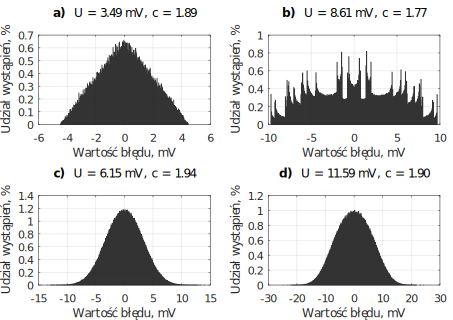
\includegraphics{obrazki/hist_part_a}
\makecaption{fig:symul_parta_hist}{Histogramy błędów \textbf{a)}~statycznego, \textbf{b)}~dynamicznego, \textbf{c)}~losowego, \textbf{d)}~wypadkowego, wielkości wyjściowej zastosowanego w eksperymencie symulacyjnym przetwornika pomiarowego}
\end{center}
\end{figure}

Wyznaczona na drodze eksperymentu niepewność $U_{a,\Sigma}$ wyniosła \qty{11.72}{mV}, przy czym współczynnik rozszerzenia $c_{a,\Sigma}$ wyniósł $1.93$. Wartość niepewności oszacowana na podstawie równania~\eqref{eq:sym_parta_uncert_value_a} jest zatem około 5\% większa od wartości uzyskanej na drodze eksperymentu, co wynika z niedoskonałości przyjętej metody wyznaczania niepewności wypadkowej \cite{jakubiec_system}. W przypadku wartości oszacowanej na podstawie równania~\eqref{eq:sym_parta_uncert_value_b} rozbieżność jest nieco mniejsza i wynosi około 2\%, co dowodzi że w analizowanym przypadku spełnione zostały założenia związane z centralnym twierdzeniem granicznym, a przyjęte uproszczenia okazały się nie mieć znaczącego wpływu na wynik obliczeń. Podobna sytuacja ma miejsce w przypadku oszacowanej wartości współczynnika rozszerzenia. Uzyskana wartość wypadkowa wariancji błędu wielkości wyjściowej wyniosła każdorazowo \qty{37.0}{\micro V}, co pokrywa się z wartością wyznaczoną w równaniu~\eqref{eq:sym_parta_var_sum} oraz tą wyznaczaną w równaniu~\eqref{eq:sym_parta_uncert_value_b}. Wyznaczone w równaniach od~\eqref{eq:sym_parta_uncert_stat} do~\eqref{eq:sym_parta_var_dyn} parametry dla składowych błędu statycznego, dynamicznego i losowego również pokrywają się z tymi wyznaczonymi na drodze eksperymentu.

Zaproponowana w pracy \cite{jakubiec_system} metoda wyznaczania niepewności wypadkowej, mimo uwzględniania założeń wynikających z centralnego twierdzenia granicznego, zgodnie z uwagami zawartymi w jej opisie, zapewnia wyniki zawyżone o kilka procent w stosunku do wartości uzyskiwanych symulacyjne. Jako, że omawiane rozbieżności są niewielkie oraz ich znak jest dodatni, uzyskiwane wyniki można uznać za prawidłowe. Wadą przedstawionej metody jest jednak konieczność wyznaczania współczynników koherencji, których wartości zależą zarówno od kształtu splatanych rozkładów, jak i od ich wariancji. Wada ta powoduje, że dla rozkładów o niestandardowym kształcie jej obszar zastosowań staje się ograniczony. Jak wykazały przeprowadzone eksperymenty i obliczenia, splatając kilka rozkładów cechujących się wartością niepewności rozszerzonej tego samego rzędu, obliczenia można uprościć zakładając kształt rozkładu wynikowego zbliżony do kształtu rozkładu normalnego.

Wobec przedstawionych rozważań i przeprowadzonego eksperymentu można stwierdzić, że zaproponowany model błędu odpowiednio opisuje związki pomiędzy kolejnymi błędami, zachodzące w analizowanym obiekcie. Z punktu widzenia analizy całości toru pomiarowego przeprowadzony proces wyznaczania parametrów wypadkowych w przypadku grupy błędów dynamicznych oraz wyznaczanie parametrów wypadkowego błędu wielkości wyjściowej był bezzasadny i został przeprowadzony jedynie w celu weryfikacji zaproponowanej metody obliczeń. Jako, że kolejne fragmenty toro pomiarowego posiadają nieidealne właściwości dynamiczne, będą one wpływać na widmo sygnału wyjściowego błędu dynamicznego analizowanego fragmentu toru pomiarowego. W przypadku pozostałych grup błędów wyznaczenie ich parametrów wypadkowych pozwoli uprościć dalszą analizę ze względu na fakt, że cechują się one typowymi kształtami rozkładów -- w innym przypadku dalsze wyznaczanie wartości współczynników koherencji byłoby problematyczne, co pokazano w omówionym przykładzie.

\section{Analiza wzmacniacza pomiarowego}

Kolejną część toru pomiarowego stanowi wzmacniacz operacyjny, którego zadaniem jest dopasowanie poziomu sygnału napięciowego $y_{a}(t)$, reprezentującego mierzoną wielkość fizyczną $s(t)$, do zakresu napięcia wejściowego przetwornika analogowo-cyfrowego. Realizacje tego elementu stanowi wzmacniacz operacyjny w konfiguracji nieodwracającej, co dodatkowo pozytywnie wpływa na zwiększenie impedancji wejściowej tego elementu oraz zmniejszenie jego impedancji wyjściowej. Zakładane wzmocnienie układu wynosi $\qty{3.3}{V \per V}$, natomiast jego funkcję przetwarzania $\dot{f}_{b}(x)$ opisuje addytywna funkcja liniowa, przy czym:
\begin{equation}
\dot{f}_{b} \emb{x} = 3.3 \cdot x \label{eq:sym_partb_function}.
\end{equation}
Dodatkowo przyjmuje się, że nieliniowość przedstawionej charakterystyki statycznej wzmacniacza jest pomijalnie mała. Analizowany układ charakteryzować się będzie częstotliwością graniczną równą $f_{b,g} = \qty{650}{kHz}$, stąd opisać można jego transmitancje i związane z nią parametry równaniami:
\begin{equation}
\tilde{G}_{b} \emb{j\omega} = \frac{1}{1 + j \frac{\omega}{2 \pi f_{b,g}}} = \frac{1}{\frac{\omega^{2}}{4 \pi^{2} f_{b,g}^{2}} + 1} - j \frac{\omega}{2 \pi f_{b,g} \left( \frac{\omega^{2}}{4 \pi^{2} f_{b,g}^{2}} + 1 \right) } \label{eq:sym_partb_trans},
\end{equation}
a zatem równania~\eqref{eq:mid_cont_amp} oraz~\eqref{eq:mid_cont_phi} przyjmują postać:
\begin{gather}
\tilde{K}_{b} \emb{\omega} = \left( \frac{\omega^{2}}{4 \pi^{2} f_{b,g}^{2}} + 1 \right)^{-\frac{1}{2}} \label{eq:sym_partb_amp_real}, \\
\tilde{\varphi}_{b} \emb{\omega} = \arctan \left( -\frac{\omega}{2 \pi f_{b,g}} \right) \label{eq:sym_partb_phi_real},
\end{gather}
przy czym dla idealnej transmitancji $\dot{G}_{b}(j\omega)$ parametry te wynoszą kolejno:
\begin{gather}
\dot{K}_{b} \emb{\omega} = 1 \label{eq:sym_partb_amp_ideal}, \\
\dot{\varphi}_{b} \emb{\omega} = 0 \label{eq:sym_partb_phi_ideal}.
\end{gather}
Temperatura otoczenia wpływać będzie na dryf zera, zgodnie z poniższą zależnością:
\begin{equation}
f_{b,z} \left( \vartheta \emb{t} \right) = \frac{7}{2} \left( \vartheta \emb{t} - \qty{20}{\degreeCelsius} \right) ~\unit{\frac{mV}{K}} \label{eq:sym_partb_temp_err}.
\end{equation}

Można zatem, podobnie jak w ramach poprzedniego fragmentu toru pomiarowego, opisać właściwości analizowanego obiektu stosując zaproponowany w pracy model:
\begin{gather}
\dot{y}_{b} \emb{t} = f_{b} \left( \dot{y}_{a} \emb{t} \right) = 3.3 \cdot \dot{y}_{a} \emb{t} \label{eq:sym_partb_out_ideal}, \\
\tilde{y}_{b} \emb{t} = \dot{y}_{b} \emb{t} + e_{b,\Sigma} \emb{t} \label{eq:sym_partb_out_real},
\end{gather}
Na wypadkowy błąd $e_{b,\Sigma}(t)$ składać się będą błędy zawarte w przetwarzanym sygnale $y_{a}(t)$ przenoszone przez analizowany element oraz błędy własne, które wprowadzane będą przez analizowany wzmacniacz pomiarowy.

Pierwszą omawianą grupą błędów będą błędy własne, wprowadzane przez analizowany obiekt. Błąd statyczny własny, wynikający z dryfu zera spowodowanego temperaturą otoczenia, opisać można równaniem:
\begin{equation}
e_{b,sw} \emb{t} = f_{b,z} \left( \vartheta \emb{t} \right) \label{eq:sym_partb_err_sw},
\end{equation}
natomiast błąd dynamiczny własny, wynikający z nieidealnej transmitancji obiektu, dla pojedynczej harmonicznej o pulsacji $\omega$ opisuje równanie:
\begin{equation}
\begin{split}
e_{b,dw} \emb{t,\omega} = ~
& \dot{f}_{b} \left( \tilde{K}_{b} \emb{\omega} E_{a,o} \emb{\omega} \sin \left( \omega t + \varphi_{a,o} \emb{\omega} + \tilde{\varphi}_{b} \emb{\omega} \right) \right)- \\
& \dot{f}_{b} \left( \dot{K}_{b} \emb{\omega} E_{a,o} \emb{\omega} \sin \left( \omega t + \varphi_{a,o} \emb{\omega} + \dot{\varphi}_{b} \emb{\omega} \right) \right) = \\
& \dot{f}_{b} \left( \tilde{K}_{b} \emb{\omega} E_{s,o} \emb{\omega} \sin \left( \omega t + \varphi_{s,o} \emb{\omega} + \tilde{\varphi}_{b} \emb{\omega} \right) \right) - \\
& \dot{f}_{b} \left( \dot{K}_{b} \emb{\omega} E_{s,o} \emb{\omega} \sin \left( \omega t + \varphi_{s,o} \emb{\omega} + \dot{\varphi}_{b} \emb{\omega} \right) \right)
\end{split}
\label{eq:sym_partb_dyn_self_err},
\end{equation}
wynikające z zależności~\eqref{eq:mid_cont_err_dyn_self} oraz~\eqref{eq:out_cont_err_dyn_prop}, przy czym wypadkowy błąd dynamiczny własny jest określony w postaci sumy kolejnych harmonicznych sygnału błędu dynamicznego własnego i może zostać opisany w postaci:
\begin{equation}
e_{b,dw} \emb{t} = \sum _{i = 1} ^{\infty} e_{b,dw} \emb{t,\omega_{a,i}} \label{eq:sym_partb_dyn_self_sum}.
\end{equation}

Drugą grupę błędów stanowią błędy propagowane, przenoszone z wejścia na wyjście obiektu. Błędy statyczny $e_{a,sw}(t)$, związany z dryfem zera przetwornika pomiarowego, oraz losowy $e_{a,rw}$, związany z nieliniowością charakterystyki zastosowanego przetwornika pomiarowego, będą przenoszone zgodnie z następującymi zależnościami:
\begin{gather}
e_{b,sp} \emb{t} = \dot{f}_{b} \left( e_{a,sw} \emb{t} \right) = 3.3 \cdot e_{a,sw} \emb{t} \label{eq:sym_partb_stat_prop_err}, \\
e_{b,rp,1} \emb{t} = \dot{f}_{b} \left( e_{a,rw} \emb{t} \right) = 3.3 \cdot e_{a,rw} \emb{t} \label{eq:sym_partb_rand_prop_err_1}.
\end{gather}
Błąd losowy $e_{b,rp,2}$ związany z szumem obecnym w sygnale pomiarowym, z którym związany jest błąd $e_{a,rp,2}$, należy analizować zgodnie z zależnościami~\eqref{eq:mid_cont_var_rand} oraz~\eqref{eq:out_cont_err_rand_prop}. Podobnie, jak w przypadku analizowanego przetwornika pomiarowego, w zakresie częstotliwości próbkowania transmitancja obiektu nie będzie miała wpływu na widmo przetwarzanego sygnału szumu. Można zatem zapisać równanie opisujące przebieg omawianego błędu na wyjściu obiektu:
\begin{equation}
e_{b,rp,2} \emb{t} = \dot{f}_{b} \left( e_{a,rp} \emb{t} \right) = 3.3 \cdot e_{a,rp} \emb{t} \label{eq:sym_partb_rand_prop_err_2},
\end{equation}
oraz wskazać zależność opisującą sumaryczny błąd losowy propagowany analizowanego obiektu daną równaniem:
\begin{equation}
e_{b,rp} \emb{t} = e_{b,rp,1} \emb{t} + e_{b,rp,2} \emb{t} = 3.3 \left( e_{a,rp} \emb{t} + e_{a,rw} \emb{t} \right) \label{eq:sym_partb_rand_prop_err},
\end{equation}
Propagacja błędów dynamicznych $e_{a,dw}$ zawartych w przetwarzanym sygnale analizowana będzie z osobna dla każdej harmonicznej błędu dynamicznego, których parametry zestawiono w tabeli~\ref{tab:sym_parta_params_dyn_summary}. Harmoniczne te, zgodnie z charakterystyką dynamiczną analizowanego wzmacniacza, będą odpowiednio tłumione i przesuwane w fazie, a następnie zgodnie z jego charakterystyką statyczną zostaną wzmocnione. Przedstawione zależności, zgodnie z równaniami~\eqref{eq:mid_cont_err_dyn_prop} oraz~\eqref{eq:out_cont_err_dyn_prop} przyjmują postać:
\begin{gather}
e_{b,dp} \emb{t,\omega} = \dot{f}_{b} \left( \tilde{K}_{b} \emb{\omega} E_{a,e} \emb{\omega} \sin \left( \omega t + \varphi_{a,e} \emb{\omega} + \tilde{\varphi}_{b} \emb{\omega} \right) \right) \label{eq:sym_partb_dyn_prop_err},\\
e_{b,dp} \emb{t} = \sum _{i = 1} ^{\infty} e_{b,dp} \emb{t,\omega_{a,i}} \label{eq:sym_partb_dyn_prop_sum}.
\end{gather}

Na podstawie przedstawionych zależności, zgodnie z równaniem~\eqref{eq:out_cont_err_sum_add}, opisać można wypadkowy błąd wielkości wyjściowej analizowanego wzmacniacza pomiarowego w postaci równania:
\begin{equation}
e_{b,\Sigma} \emb{t} = e_{b,sw} \emb{t} + e_{b,sp} \emb{t} + e_{b,rp} \emb{t} + e_{b,dw} \emb{t} + e_{b,dp} \emb{t} \label{eq:sym_partb_error_sum}.
\end{equation}

Kolejny etap analizy sprowadza się do wyznaczenia parametrów opisanych sygnałów błędów. Jako, że proces pomiaru powtarzany będzie wielokrotnie, należy dla wskazanych sygnałów określić ich parametry w kategorii probabilistycznej, uwzględniając zachodzące pomiędzy nimi związki. W przypadku błędów dynamicznych należy, analogicznie jak w przypadku przedstawionej analizy przetwornika pomiarowego, wyznaczyć wypadkowe amplitudy i przesunięcia w fazie kolejnych harmonicznych sygnału błędu. W analizowanym przypadku każda wypadkowa harmoniczna sygnału błędu dynamicznego złożona będzie z trzech składników -- dwóch wynikających z równania~\eqref{eq:sym_partb_dyn_self_err} oraz jednej wynikającej z równania~\eqref{eq:sym_partb_dyn_prop_err}. Parametry wypadkowe należy wyznaczyć zgodnie z metodą opisaną w równaniach od~\eqref{eq:dyn_vect} do~\eqref{eq:dyn_vect_phi}. W przypadku pozostałych błędów składowych należy określić ich wariancję uwzględniając funkcję przetwarzania obiektu, przy czym w przypadku liniowej i addytywnej funkcji przetwarzania zapisać można zależność:
\begin{equation}
\sigma_{wy}^{2} = f \emb{\sigma_{we}}^{2} \label{eq:var_function},
\end{equation}
gdzie $\sigma_{wy}^{2}$ jest wariancją na wyjściu funkcji przetwarzania $f(x)$, a $\sigma_{we}^{2}$ wariancją na wejściu. Dodatkowo zauważyć należy, że kształt rozkładu przetwarzanej wielkości nie ulega zmianie. Wyznaczone analogicznie do przykładu opisanego w równaniach od~\eqref{eq:sym_parta_dyn_self_example_sum} do~\eqref{eq:sym_parta_dyn_self_example_phi} parametry wypadkowe sygnału błędu dynamicznego $e_{b,d}$ zestawiono w tabeli~\ref{tab:sym_partb_params_dyn_summary}, natomiast tabela~\ref{tab:sym_partb_params_unc_list} przedstawia budżet niepewności wielkości wyjściowej analizowanego wzmacniacza pomiarowego z uwzględnieniem podziału na błędy własne i propagowane.

\begin{table}[htb!]
\begin{center}
\makecaption{tab:sym_partb_params_dyn_summary}{Parametry wypadkowe kolejnych harmonicznych błędu dynamicznego analizowanego w eksperymencie symulacyjnym wzmacniacza pomiarowego}
\begin{tabular}[c]{| c | c | S[table-format = 2.2] | S[table-format = +1.2] |} \hline
\textbf{Lp. $j$} & \textbf{Pulsacja $\omega_{b,j}$, rad/s} & \textbf{Amplituda $E_{b,e}(\omega_{b,j})$, mV} & \textbf{Faza $\varphi_{b,e}(\omega_{b,j})$, rad} \\ \hline
1 & $1000  \cdot 2\pi$  &   9.23  & -1.57  \\ \hline
2 & $5000  \cdot 2\pi$  &  23.08  &  1.96  \\ \hline
3 & $15000 \cdot 2\pi$  &  23.07  & -1.07  \\ \hline
\end{tabular}
\end{center}
\end{table}

\begin{table}[htb!]
\begin{center}
\makecaption{tab:sym_partb_params_unc_list}{Budżet niepewności wielkości wyjściowej analizowanego w eksperymencie symulacyjnym wzmacniacza pomiarowego, gdzie (a) oznacza przetwornik pomiarowy oraz (b) oznacza wzmacniacz pomiarowy}
\begin{tabular}[c]{| c | c | S[table-format = 2.2] | S[table-format = 3.2] | c | c |} \hline
\textbf{Lp.} & \textbf{Symbol} & \textbf{$U_{95\%}$, mV} & \textbf{$\sigma^{2}$, \micro V} & \textbf{Rozkład} & \textbf{Źródło błędu} \\ \hline
1  & ${b,sw}$       & 11.52 &  36.75  & trójkątny                    & dryf temperatury (a)                       \\ \hline
2  & ${b,sp}$       & 8.15  &  18.38  & trójkątny                    & dryf temperatury (b)                       \\ \hline
3  & ${b,rp,1}$     & 9.93  &  36.26  & jednostajny                  & nieliniowość obiektu (a)                   \\ \hline
4  & ${b,rp,2}$     & 16.70 &  72.64  & normalny                     & szum wielkości wejściowej                  \\ \hline
5  & ${b,dp,1}$     & 6.21  &  19.14  & \multirow{6}{*}{dwumodalny}  & \multirow{3}{*}{transmitancja (a)}         \\ \cline{1-4}
6  & ${b,dp,2}$     & 15.53 &  119.62 &                              &                                            \\ \cline{1-4}
7  & ${b,dp,3}$     & 15.52 &  119.44 &                              &                                            \\ \cline{1-4} \cline{6-6}
8  & ${b,dw,1}$     & 3.06  &  4.64   &                              & \multirow{3}{*}{transmitancja (b)}         \\ \cline{1-4}
9  & ${b,dw,2}$     & 7.65  &  29.00  &                              &                                            \\ \cline{1-4}
10 & ${b,dw,3}$     & 7.65  &  28.99  &                              &                                            \\ \hline
\end{tabular}
\end{center}
\end{table}

Ostatnim krokiem analizy pozostaje określenie związków pomiędzy składowymi budżetu niepewności zestawionymi w tabeli~\ref{tab:sym_partb_params_unc_list}. Należy zauważyć, że składowe związane z dryfem temperaturowym przetwornika pomiarowego oraz dryfem temperaturowym wzmacniacza zależą od tej samej wielkości fizycznej -- temperatury otoczenia. Oznacza to, że należy określić korelacje pomiędzy omawianymi wielkościami zgodnie z zależnością~\eqref{eq:var_corr} i uwzględnić ją w równaniu~\eqref{eq:var_matrix} w celu określenia wypadkowej wariancji składanych sygnałów błędu. Wyznaczony współczynnik korelacji pomiędzy opisywanymi błędami statycznymi wynosi:
\begin{equation}
r_{b,sw,sp} = \frac{\sigma_{b,sw,sp}^{2} - \sigma_{b,sw}^{2} - \sigma_{b,sp}^{2}}{2 \sigma_{b,sw} \sigma_{b,sp}} = \frac{\num{1.07e-4} - \num{3.68e-5} - \num{1.84e-5}}{2 \cdot \num{6.06e-3} \cdot \num{4.29e-3}} = 1.00 \label{eq:sym_partb_stat_corr},
\end{equation}
przy czym w celu wyznaczenia wypadkowej wartości wariancji $\sigma_{b,sw,sp}^{2}$ przeprowadzono eksperyment metodą Monte-Carlo. Ze względu na fakt, że analizowane sygnały błędu statycznego zależą liniowo w pełni od tej samej wielkości fizycznej, rozkład błędu wypadkowego cechować się będzie kształtem identycznym, jak rozkład omawianej wielkości fizycznej. W przypadku kolejnych harmonicznych błędu dynamicznego własnego oraz propagowanego zauważyć można, że przesunięcia fazowe przebiegów tych harmonicznych są pomijalnie małe -- ich rząd wielkości wynosi \qty{1e-3}{rad}. Można zatem przyjąć, że współczynniki korelacji składanych sygnałów będą zbliżone do jedności, co pozwoli zastosować równanie~\eqref{eq:var_matrix} do określenia wypadkowej wariancji tych przebiegów. Założenia te potwierdzają wyniki zestawione w tabeli~\ref{tab:sym_partb_params_dyn_summary}.

Korzystając zależności przedstawionych równaniami od~\eqref{eq:sym_parta_uncert_stat} do~\eqref{eq:sym_parta_var_dyn}, równania~\eqref{eq:var_function} oraz zestawionych w tabeli~\ref{tab:sym_partb_params_unc_list} wartości, wyznaczono budżet niepewności uwzględniający podział na kategorie błędów, przy czym ze względu na konieczność przeprowadzania dalszej analizy w dziedzinie pulsacji, nie wyznaczano wypadkowych parametrów błędu dynamicznego. Wyznaczone wartości przedstawia tabela~\ref{tab:sym_partb_params_unc_sum}, która zostanie wykorzystana w dalszym etapie analizy toru pomiarowego.

\begin{table}[htb!]
\begin{center}
\makecaption{tab:sym_partb_params_unc_sum}{Budżet niepewności wielkości wyjściowej analizowanego w eksperymencie symulacyjnym wzmacniacza pomiarowego z uwzględnieniem podziału na błędy statyczne, dynamiczne oraz losowe}
\begin{tabular}[c]{| c | c | S[table-format = 2.2] | S[table-format = 3.2] | c | c |} \hline
\textbf{Lp.} & \textbf{Symbol} & \textbf{$U_{95\%}$, mV} & \textbf{$\sigma^{2}$, \micro V} & \textbf{Rozkład} & \textbf{Źródło błędu} \\ \hline
1 & ${b,s}$        & 19.66 &  107.01 & trójkątny                    & wypadkowy dryf temperatury                 \\ \hline
2 & ${b,r}$        & 20.45 &  108.90 & normalny                     & szum i nieliniowość obiektu                \\ \hline
3 & ${b,d,1}$      & 9.20  &  42.60  & \multirow{3}{*}{dwumodalny}  & \multirow{3}{*}{wypadkowa transmitancja}   \\ \cline{1-4}
4 & ${b,d,2}$      & 23.01 &  266.34 &                              &                                            \\ \cline{1-4}
5 & ${b,d,3}$      & 23.00 &  266.11 &                              &                                            \\ \hline
\end{tabular}
\end{center}
\end{table}

W celu weryfikacji poprawności zastosowanego modelu błędu oraz przeprowadzonych obliczeń wykonano eksperyment metodą Monte-Carlo, polegający na wyznaczeniu sto tysięcy razy wartości wielkości wyjściowej analizowanego wzmacniacza pomiarowego. Podczas eksperymentu fazę sygnału wejściowego $s(t)$ losowano z przedziału $<-2 \pi f_{1};2 \pi f_{1}>\unit{rad}$, przy czym wylosowanie każdej w możliwych wartości było jednakowo prawdopodobne. Uzyskiwaną wartość wielkości wyjściowej porównywano z wartością otrzymaną dla idealnej realizacji analizowanego fragmentu toru pomiarowego (tj. takiej, w której nie występowały żadne źródła błędów), a następnie na podstawie równania~\eqref{eq:sym_partb_error_sum} wyznaczano realizację błędu wielkości wyjściowej $y_{b}(t)$. Wyznaczone wartości zostały użyte do sporządzenia histogramu, na podstawie którego określono parametry rozkładu błędu analizowanej wielkości wyjściowej. Eksperyment wykonano uwzględniając wszystkie źródła błędu oraz uwzględniając źródła związane z kolejnymi kategoriami błędów. Uzyskane na drodze eksperymentu histogramy przedstawia rysunek~\ref{fig:symul_partb_hist}.

\begin{figure}[htb!]
\begin{center}
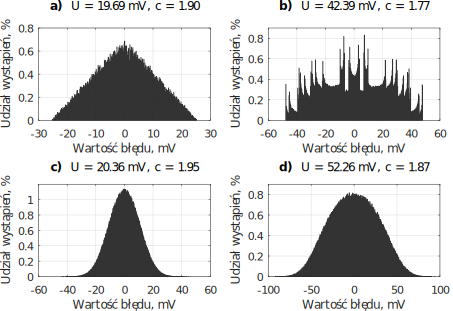
\includegraphics{obrazki/hist_part_b}
\makecaption{fig:symul_partb_hist}{Histogramy błędów \textbf{a)}~statycznego, \textbf{b)}~dynamicznego, \textbf{c)}~losowego, \textbf{d)}~wypadkowego, wielkości wyjściowej zastosowanego w eksperymencie symulacyjnym wzmacniacza pomiarowego}
\end{center}
\end{figure}

Analizując wyniki eksperymentu zauważyć można, że uzyskane wyniki dla błędów losowego oraz statycznego są zbliżone do tych przedstawionych w tabeli~\ref{tab:sym_partc_params_unc_sum}. Pozwala to zakładać, że podobnie jak w przypadku analizy właściwości przetwornika pomiarowego, przyjęty model błędu oraz stosowane zależności poprawnie określają związki pomiędzy wskazanymi błędami i umożliwiają poprawne oszacowanie ich parametrów. Na etapie przeprowadzonej analizy nie wyznaczano wypadkowych parametrów błędu dynamicznego oraz całkowitego błędu wypadkowego -- dane te, jak pokazano na obecnym przykładzie, nie są użyteczne podczas analizy kolejnych fragmentów toru pomiarowego, przy czym ich wyznaczenie wymaga pewnego nakładu obliczeń.

\section{Analiza przetwornika analogowo-cyfrowego}

Kolejnym elementem wchodzącym w skład analizowanego toru pomiarowego jest przetwornik analogowo-cyfrowy. W eksperymencie zakłada się, że element jest realizowany przy użyciu 8-bitowego przetwornika wagowego o zakresie napięcia wejściowego z przedziału $<-3;3>\unit{V}$. Wobec powyższych liczba dostępnych wartości wielkości wyjściowej tego przetwornika wynosi $N_{q} = 256$, natomiast wartość kwantu jest równa $q = \frac{3 - (-3) ~\unit{V}}{256} = \qty{23.44}{mV}$. Zakładając, że wielkością wyjściową $x_{c}(n)$ analizowanego przetwornika będzie dyskretna reprezentacja wielkości wejściowej $y_{b}(t)$, zapisać można następujące zależności:
\begin{gather}
\dot{x}_{c} \emb{n} = \dot{y}_{b} \emb{nT_{p}} \label{eq:sym_partc_out_ideal}, \\
\tilde{x}_{c} \emb{n} = \tilde{y}_{b} \emb{nT_{p}} + e_{c,q} \left( \tilde{y}_{b} \emb{nT_{p}} \right) = \dot{x}_{c} \emb{n} + e_{c,\Sigma} \emb{n} \label{eq:sym_partc_out_real}, \\
e_{c,\Sigma} \emb{n} = e_{b,\Sigma} \emb{nT_{p}} + e_{c,q} \left( \tilde{y}_{b} \emb{nT_{p}} \right) \label{eq:sym_partc_error_sum},
\end{gather}
gdzie $T_{p}$ jest okresem próbkowania równym $\frac{1}{\qty{48}{kHz}} = \qty{20.8(3)}{\micro s}$.
Na podstawie zależności danych równaniami od~\eqref{eq:adc_function} do~\eqref{eq:adc_qerrrange} zapisać można nierówność określającą przedział, w jakim znajdować się będzie błąd kwantowania $e_{c,q}(x)$ jako:
\begin{equation}
\qty{-11.72}{mV} \le e_{c,q} \emb{x} \le \qty{11.72}{mV} \label{eq:sym_partc_error_quant}.
\end{equation}

Analizując równanie~\eqref{eq:sym_partc_out_real} zauważyć można, że realizacja błędu kwantowania zależna jest od wartości przetwarzanej wielkości wejściowej analizowanego przetwornika. Jednakże, jak wykazano w pracach \cite{sienkowski_kwant, sienkowski_adc}, zależność tą można pominąć. Przy założeniu, że uzyskanie na wejściu przetwornika dowolnej wartości z zakresu wartości wielkości wejściowej jest jednakowo prawdopodobne oraz że podczas pomiaru wielkość ta będzie się zmieniać, powtarzając proces pomiaru wielokrotnie, z punktu widzenia pojedynczego okna pomiarowego błąd kwantowania $e_{c,q}(x)$ rozpatrywać można w kategoriach probabilistycznych jako losową realizację wielkości z zakresu opisanego równaniem~\eqref{eq:sym_partc_error_quant} o rozkładzie jednostajnym \cite{jakubiec_system}. Takie podejście umożliwia zastosowanie zaproponowanego w pracy modelu błędu, podczas gdy analiza zakładająca funkcję przetwarzania omawianego obiektu daną w postaci równania~\eqref{eq:adc_output} byłaby skomplikowana. Wobec powyższych założeń wariancja $\sigma_{c,q}^{2}$ oraz niepewność rozszerzona $U_{c,q}$ związane z błędem kwantowania $e_{c,q}(x)$ mogą być opisane przez następujące zależności:
\begin{gather}
\sigma_{c,q}^{2} = \frac{ q^{2}}{12} = \frac{\emb{\num{23.44e-3}}^{2} }{12} = \qty{45.78}{\micro V} \label{eq:sym_partc_var_quant}, \\
U_{c,q} = c_{u} \sigma_{c,q} = 1.65 \cdot \num{6.77e-3} = \qty{11.16}{mV} \label{eq:sym_partc_uncert_quant}.
\end{gather}

Aby zweryfikować poprawność przedstawionych zależności przeprowadzono eksperyment stosując metodę Monte-Carlo. W ramach eksperymentu wyznaczono sto tysięcy razy realizację wartości wielkości wyjściowej analizowanego przetwornika analogowo-cyfrowego, a następnie jej wartość porównano z wartością idealną, uzyskaną dla toru pomiarowego w którym nie występowały żadne źródła błędów. Na podstawie uzyskanych zgodnie z równaniem~\eqref{eq:sym_partc_error_sum} realizacji błędu opracowano histogram i określono jego parametry. Identyczny eksperyment przeprowadzono ponownie, z tą różnicą, że jako jedyne źródło błędów, uwzględniono w nim jedynie obecność procesu kwantowania w celu oszacowania jedynie parametrów błędu kwantowania. Rysunek~\ref{fig:symul_partc_hist} przedstawia uzyskane na drodze eksperymentu histogramy.

\begin{figure}[htb!]
\begin{center}
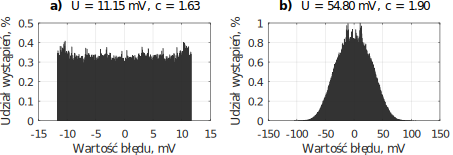
\includegraphics{obrazki/hist_part_c}
\makecaption{fig:symul_partc_hist}{Histogramy błędów \textbf{a)}~kwantowania, \textbf{b)}~wypadkowego, wielkości wyjściowej zastosowanego w eksperymencie symulacyjnym przetwornika analogowo-cyfrowego}
\end{center}
\end{figure}

Analizując wyniki poprzedniego eksperymentu przedstawione na rysunku~\ref{fig:symul_partb_hist} oraz wyniki bieżącego eksperymentu przedstawione na rysunku~\ref{fig:symul_partc_hist}, wnioskować można że zaproponowane wcześniej założenia są spełnione. Wariancja błędu wypadkowego $\sigma_{b,\Sigma}^{2}$ wielkości wejściowej przetwornika analogowo-cyfrowego wyniosła w poprzednim eksperymencie około \qty{787}{\micro V}. Wariancja błędu wypadkowego $\sigma_{c,\Sigma}^{2}$ wielkości wyjściowej przetwornika analogowo-cyfrowego wyniosła w bieżącym eksperymencie około \qty{832}{\micro V}. Wartość wariancji błędu kwantowania $\sigma_{c,q}^{2}$ uzyskana na drodze eksperymentu wyniosła \qty{46.79}{\micro V}, a związana z nią niepewność $U_{c,q}$ wyniosła \qty{11.15}{mV}, co w zadowalającym stopniu pokrywa się z wartościami wyznaczonymi na podstawie równań~\eqref{eq:sym_partc_var_quant} oraz~\eqref{eq:sym_partc_uncert_quant}. Przedstawione wartości pozwolą określić korelacje pomiędzy wariancją błędu wypadkowego wielkości wejściowej przetwornika analogowo-cyfrowego oraz błędu kwantowania na podstawie równania~\eqref{eq:var_corr}, które w omawianym przypadku przyjmuje postać:
\begin{equation}
r_{c,q;b,\Sigma} = \frac{\sigma_{c,\Sigma}^{2} - \sigma_{c,q}^{2} - \sigma_{b,\Sigma}^{2}}{2 \sigma_{c,q} \sigma_{b,\Sigma}} = \frac{\num{8.31e-4} - \num{4.68e-5} - \num{7.87e-4}}{2 \cdot \num{6.84e-3} \cdot \num{2.81e-2}} = \num{-7.3e-3} \label{eq:sym_partc_corr}.
\end{equation}

Uzyskana wartość współczynnika korelacji oraz wyniki przeprowadzonych eksperymentów świadczą o prawidłowości przyjętych założeń i pomijalnie małej korelacji błędu kwantowania z przebiegiem przetwarzanego przez analizowany obiekt sygnału oraz zawartych w nim sygnałów błędów. Na podstawie przedstawionych zależności oraz tabeli~\ref{tab:sym_partb_params_unc_list} sporządzić można kompletny budżet niepewności wielkości wyjściowej $x_{c}(n)$ analizowanego przetwornika analogowo-cyfrowego, który zestawiono w tabeli~\ref{tab:sym_partc_params_unc_list}. Ze względu na możliwość pominięcia wpływu opisywanych oraz zależności określone równaniami od~\eqref{eq:sym_partc_out_ideal} do~\eqref{eq:sym_partc_error_sum} założyć można, że przenoszone z wejścia na wyjście analizowanego obiektu sygnały błędów przenoszone będą w stosunku 1:1, a zatem zachowają one swoje oryginalne parametry oraz zostaną opisane jako błędy propagowane.

\begin{table}[htb!]
\begin{center}
\makecaption{tab:sym_partc_params_unc_list}{Budżet niepewności wielkości wyjściowej analizowanego w eksperymencie symulacyjnym przetwornika analogowo-cyfrowego, gdzie (a) oznacza przetwornik pomiarowy, (b) oznacza wzmacniacz pomiarowy oraz (c) oznacza przetwornik analogowo-cyfrowy}
\begin{tabular}[c]{| c | c | S[table-format = 2.2] | S[table-format = 3.2] | c | c |} \hline
\textbf{Lp.} & \textbf{Symbol} & \textbf{$U_{95\%}$, mV} & \textbf{$\sigma^{2}$, \micro V} & \textbf{Rozkład} & \textbf{Źródło błędu} \\ \hline
1  & ${c,rw,q}$     & 11.16 &  45.78  & jednostajny                  & proces kwantowania (c)                     \\ \hline
2  & ${c,sp,1}$     & 11.52 &  36.75  & trójkątny                    & dryf temperatury (a)                       \\ \hline
3  & ${c,sp,2}$     & 8.15  &  18.38  & trójkątny                    & dryf temperatury (b)                       \\ \hline
4  & ${c,rp,1}$     & 9.93  &  36.26  & jednostajny                  & nieliniowość obiektu (a)                   \\ \hline
5  & ${c,rp,2}$     & 16.70 &  72.64  & normalny                     & szum wielkości wejściowej                  \\ \hline
6  & ${c,dp,a,1}$   & 6.21  &  19.14  & \multirow{6}{*}{dwumodalny}  & \multirow{3}{*}{transmitancja (a)}         \\ \cline{1-4}
7  & ${c,dp,a,2}$   & 15.53 &  119.62 &                              &                                            \\ \cline{1-4}
8  & ${c,dp,a,3}$   & 15.52 &  119.44 &                              &                                            \\ \cline{1-4} \cline{6-6}
9  & ${c,dp,b,1}$   & 3.06  &  4.64   &                              & \multirow{3}{*}{transmitancja (b)}         \\ \cline{1-4}
10 & ${c,dp,b,2}$   & 7.65  &  29.00  &                              &                                            \\ \cline{1-4}
11 & ${c,dp,b,3}$   & 7.65  &  28.99  &                              &                                            \\ \hline
\end{tabular}
\end{center}
\end{table}

Przedstawiony w tabeli~\ref{tab:sym_partc_params_unc_list} budżet niepewności dobrze obrazuje źródła błędów występujące w analizowanym torze pomiarowym oraz jednoznacznie wskazuje ich parametry. Na dalszym etapie analizy stosowanie przedstawionego zestawienia jest jednak kłopotliwe, ponieważ wiązać się będzie z koniecznością osobnej analizy każdego z wskazanych sygnałów błędu z osobna. Ze względu na fakt, że proponowany w pracy model błędu dotyczący kolejnego fragmentu toru pomiarowego, jakim jest algorytm transformacji falkowej, wymaga jedynie określenia wariancji wypadkowego błędu statycznego, losowego oraz wariancji kolejnych wypadkowych harmonicznych błędu dynamicznego, podobnie jak to miało miejsce w przypadku poprzedniego elementu analizowanego toru pomiarowego przedstawiony zostanie budżet niepewności uwzględniający opisywany podział. Biorąc pod uwagę przedstawione w bieżącym podrozdziale założenia oraz wyniki zawarte w tabeli~\ref{tab:sym_partb_params_unc_sum}, sporządzono budżet niepewności z uwzględnieniem omawianego podziału, który zestawiono w tabeli~\ref{tab:sym_partc_params_unc_sum}. Parametry opisujące wypadkowy błąd losowy wyznaczono zgodnie z zależnościami:
\begin{gather}
\sigma_{c,r}^{2} = \sigma_{c,rp,1}^{2} + \sigma_{c,rp,2}^{2} + \sigma_{c,q}^{2} = \sigma_{b,rp,1}^{2} + \sigma_{b,rp,2}^{2} + \sigma_{c,q}^{2} = \qty{154.68}{\micro V} \label{eq:sym_partc_var_random}, \\
U_{c,r} = c_{n} \sigma_{c,r} = 1.96 \cdot \num{12.44e-3} = \qty{24.38}{mV} \label{eq:sym_partc_uncert_random},
\end{gather}
przyjmując omawiane wcześniej uproszczenie zakładające normalny rozkład wypadkowego błędu losowego.

\begin{table}[htb!]
\begin{center}
\makecaption{tab:sym_partc_params_unc_sum}{Budżet niepewności wielkości wyjściowej analizowanego w eksperymencie symulacyjnym wzmacniacza przetwornika analogowo-cyfrowego z uwzględnieniem podziału na błędy statyczne, dynamiczne oraz losowe}
\begin{tabular}[c]{| c | c | S[table-format = 2.2] | S[table-format = 3.2] | c | c |} \hline
\textbf{Lp.} & \textbf{Symbol} & \textbf{$U_{95\%}$, mV} & \textbf{$\sigma^{2}$, \micro V} & \textbf{Rozkład} & \textbf{Źródło błędu} \\ \hline
1 & ${c,s}$        & 19.66 &  107.01 & trójkątny                    & wypadkowy dryf temperatury                 \\ \hline
2 & ${c,r}$        & 24.38 &  154.68 & normalny                     & szum, nieliniowość, konwersja              \\ \hline
3 & ${c,d,1}$      & 9.20  &  42.60  & \multirow{3}{*}{dwumodalny}  & \multirow{3}{*}{wypadkowa transmitancja}   \\ \cline{1-4}
4 & ${c,d,2}$      & 23.01 &  266.34 &                              &                                            \\ \cline{1-4}
5 & ${c,d,3}$      & 23.00 &  266.11 &                              &                                            \\ \hline
\end{tabular}
\end{center}
\end{table}

\section{Analiza algorytmu transformacji falkowej}

Ostatnim fragmentem analizowanego toru pomiarowego, a za razem najistotniejszym obiektem z punktu widzenia niniejszej pracy, jest algorytm transformacji falkowej. Zakłada się, że zastosowany algorytm jest algorytmem dyskretnej transformacji falkowej, na którego wejście podawać należy wektor wielkości wejściowych $\mathbf{x}_{d}$, złożony z kolejnych $N = 8$ próbek wielkości wyjściowych $x_{c}(n)$ przetwornika analogowo-cyfrowego. Na wyjściu algorytmu każdorazowo wypracowany zostaje wektor $\mathbf{X}$ zawierający $M = 8$ wielkości wyjściowych algorytmu, które stanowić będą ostateczne wielkości wyjściowe analizowanego toru pomiarowego. Omawiany algorytm wykorzystywać będzie falkę \enquote{db2}, przy czym na jego realizację składać się będą dwie iteracje procesu dekompozycji sygnału. Macierz transformacji $\mathbf{A}$ omawianego algorytmu przedstawia równanie~\eqref{eq:db2_2_8_matrix}. Implementacja stosowanego algorytmu wykorzystywać będzie liczby zmiennoprzecinkowe o długości słowa 16-bitów.

Wobec powyższych założeń oraz modelu zaproponowanego w równaniach od~\eqref{eq:alg_out_mat} do~\eqref{eq:alg_out_single} wektor wielkości wejściowych analizowanego algorytmu opisać można w postaci:
\begin{gather}
\dot{\mathbf{x}}_{d}^{T} \emb{k} =
\begin{bmatrix}
\dot{x}_{c} \emb{kT_{p}} & \dot{x}_{c} \left( \emb{k+1} T_{p} \right) & \hdots & \dot{x}_{c} \left( \emb{k+7} T_{p} \right)
\end{bmatrix}
\label{eq:sym_partd_input_ideal}, \\
\tilde{\mathbf{x}}_{d}^{T} \emb{k} =
\begin{bmatrix}
\tilde{x}_{c} \emb{kT_{p}} & \tilde{x}_{c} \left( \emb{k+1} T_{p} \right) & \hdots & \tilde{x}_{c} \left( \emb{k+7} T_{p} \right)
\end{bmatrix}
\label{eq:sym_partd_input_real},
\end{gather}
natomiast wektor błędu wypadkowego wielkości wyjściowych algorytmu opisuje równanie:
\begin{equation}
\mathbf{e}_{d,\Sigma}^{T} \emb{k} =
\begin{bmatrix}
e_{c,\Sigma} \emb{kT_{p}} & e_{c,\Sigma} \left( \emb{k+1} T_{p} \right) & \hdots & e_{c,\Sigma} \left( \emb{k+7} T_{p} \right)
\end{bmatrix}
\label{eq:sym_partd_input_error_sum}.
\end{equation}
Dodatkowo zdefiniować można wektory błędów rozpatrując zaproponowany podział na błędy statyczne, losowe oraz dynamiczne:
\begin{gather}
\mathbf{e}_{d,s}^{T} \emb{k} =
\begin{bmatrix}
e_{c,s} \emb{kT_{p}} & e_{c,s} \left( \emb{k+1} T_{p} \right) & \hdots & e_{c,s} \left( \emb{k+7} T_{p} \right)
\end{bmatrix}
\label{eq:sym_partd_input_error_stat}, \\
\mathbf{e}_{d,r}^{T} \emb{k} =
\begin{bmatrix}
e_{c,r} \emb{kT_{p}} & e_{c,r} \left( \emb{k+1} T_{p} \right) & \hdots & e_{c,r} \left( \emb{k+7} T_{p} \right)
\end{bmatrix}
\label{eq:sym_partd_input_error_rand}, \\
\mathbf{e}_{d,d}^{T} \emb{k} =
\begin{bmatrix}
e_{c,d} \emb{kT_{p}} & e_{c,d} \left( \emb{k+1} T_{p} \right) & \hdots & e_{c,d} \left( \emb{k+7} T_{p} \right)
\end{bmatrix}
\label{eq:sym_partd_input_error_dyn},
\end{gather}
a także w analogiczny sposób rozpatrywać można wektory błędów cząstkowych, których parametry zestawiono w tabeli~\ref{tab:sym_partc_params_unc_list}. Wobec powyższego, zgodnie z równaniem~\eqref{eq:alg_out_mul}, wektor wielkości wyjściowych opisać można jako:
\begin{gather}
\dot{\mathbf{X}} \emb{k} = \mathbf{A} \cdot \dot{\mathbf{x}}_{d} \emb{k} \label{eq:sym_partd_output_ideal}, \\
\tilde{\mathbf{X}} \emb{k} = \mathbf{A} \cdot \tilde{\mathbf{x}}_{d} \emb{k} \label{eq:sym_partd_output_real},
\end{gather}
natomiast kolejne wektory błędów wielkości wyjściowej są opisane zależnościami przedstawionymi jako:
\begin{gather}
\mathbf{e}_{X,\Sigma} \emb{k} = \mathbf{A} \cdot \mathbf{e}_{d,\Sigma} \emb{k} \label{eq:sym_partd_output_error_sum}, \\
\mathbf{e}_{X,s} \emb{k} = \mathbf{A} \cdot \mathbf{e}_{d,s} \emb{k} \label{eq:sym_partd_output_error_stat}, \\
\mathbf{e}_{X,r} \emb{k} = \mathbf{A} \cdot \mathbf{e}_{d,r} \emb{k} \label{eq:sym_partd_output_error_rand}, \\
\mathbf{e}_{X,d} \emb{k} = \mathbf{A} \cdot \mathbf{e}_{d,d} \emb{k} \label{eq:sym_partd_output_error_dyn}.
\end{gather}
Należy zauważyć, że tak jak w przypadku wektora wielkości wejściowych, tak i w przypadku wektora wielkości wyjściowych, wyróżnić można również osobne wektory błędu dla każdego z opisanych w tabeli~\ref{tab:sym_partc_params_unc_list} sygnałów. Zgodnie z oznaczeniami przyjętymi w równaniach~\eqref{eq:db2_invect} oraz~\eqref{eq:db2_outvect}, wektory wielkości wejściowych i wyjściowych pojedynczej realizacji algorytmu będą w dalszej części rozdziału oznaczone symbolami:
\begin{gather}
\mathbf{x}_{d}^{T} =
\begin{bmatrix}
S_{0,0} & S_{0,1} & S_{0,2} & S_{0,3} & S_{0,4} & S_{0,5} & S_{0,6} & S_{0,7}
\end{bmatrix}
\label{eq:sym_partd_invect}, \\
\mathbf{X}^{T} =
\begin{bmatrix}
S_{2,0} & S_{2,1} & T_{2,0} & T_{2,1} & T_{1,0} & T_{1,1} & T_{1,2} & T_{1,3}
\end{bmatrix}
\label{eq:sym_partd_outvect},
\end{gather}
natomiast wektor błędów wielkości wyjściowej pojedynczej realizacji algorytmu będzie oznaczany w postaci:
\begin{equation}
\mathbf{e}_{X,*}^{T} =
\begin{bmatrix}
e_{S_{2,0},*} & e_{S_{2,1},*} & e_{T_{2,0},*} & e_{T_{2,1},*} & e_{T_{1,0},*} & e_{T_{1,1},*} & e_{T_{1,2},*} & e_{T_{1,3},*}
\end{bmatrix}
\label{eq:sym_partd_errvect},
\end{equation}
gdzie w miejsce symbolu \enquote{$*$} umieszczany będzie symbol analizowanego sygnału błędu.

W poprzednich podrozdziałach przedstawiono różne sposoby wyznaczania budżetu niepewności, uwzględniające każde źródło błędu z osobna oraz wskazujące wypadkowe parametry danego rodzaju błędu. Zabiegi te miały na celu wskazanie optymalnej drogi analizy właściwości metrologicznych z punktu widzenia projektanta toru pomiarowego, w zależności od jego intencji i potrzeb. Opisywany zabieg został również przeprowadzony w celu weryfikacji postawionej w pracy tezy, jako przy wykorzystaniu zaproponowanej metody analizy istnieje możliwość wyznaczenia jedynie zastępczych parametrów sygnałów błędów wielkości wejściowej algorytmu dyskretnej transformacji falkowej w celu oszacowania niepewności na wyjściu tego algorytmu. W dalszej części rozdziału opisane zostaną dwa sposoby wyznaczenia niepewności wielkości wyjściowych algorytmu. Podejście pierwsze uwzględniać będzie budżet niepewności podzielony na kategorie błędów, opisany w tabeli~\ref{tab:sym_partc_params_unc_sum}, natomiast podejście drugie przedstawi analizę z wykorzystaniem budżetu sporządzonego dla każdego sygnału błędu z osobna, który przedstawiono w tabeli~\ref{tab:sym_partc_params_unc_list}.

Istotnym faktem podczas analizy właściwości metrologicznych stosowanego algorytmu jest to, że jego wielkości wejściowe każdorazowo pochodzą z tego samego źródła. Powtarzając proces wyznaczania wartości wektora wielkości wyjściowych algorytmu wielokrotnie wszystkie wielkości wejściowe algorytmu cechowały będą te same parametry wariancji i niepewności rozszerzonej. Zjawisko to zostało omówione w poprzedniej części pracy. Ze względu na fakt, że w przypadku błędów o charakterze statycznym wartości realizacji tych błędów nie zmieniają się w obrębie pojedynczego okna pomiarowego, do oceny wariancji wyjściowego sygnału błędu związanego z tym rodzajem błędu stosowane będzie równanie~\eqref{eq:alg_outvar_stat}. Dla określenia parametrów rozkładu błędów o charakterze dynamicznym wykorzystana zostanie transmitancja pojedynczej wielkości wyjściowej algorytmu dana równaniem~\eqref{eq:alg_trans_single}, natomiast w przypadku błędów o charakterze losowym wykorzystywana będzie w tym celu zależność~\eqref{eq:alg_outvar_rand}.

Przedstawiane w dalszej części obliczenia dotyczyć będą dwóch przykładowych wielkości wyjściowych algorytmu -- $S_{2,0}$ oraz $T_{1,0}$. Wybór przedstawionych wielkości jest uzasadniony faktem, że jedna z nich stanowi detale sygnału (jest reprezentowana przez filtr dolno-przepustowy związany z funkcją skalującą), natomiast druga stanowi aproksymacje sygnału (jest reprezentowana przez filtr pasmowo-przepustowy związany z falką-matką). Pozostałe wielkości zostaną poddane analizie w identyczny sposób, natomiast dla zachowania czytelności obliczenia te nie będą przedstawiane w pracy.

Zgodnie z równaniem~\eqref{eq:alg_trans_single} oraz postacią macierzy $\mathbf{A}$ daną równaniem~\eqref{eq:db2_2_8_matrix}, transmitancje algorytmu związane z omawianymi wielkościami wyjściowymi przedstawiają równania:
\begin{gather}
\begin{split}
H_{S_{2,0}} \emb{z} = ~
& \frac{5 - \sqrt{3}}{16} + \frac{5 + \sqrt{3}}{16} z^{-1} + \frac{3 + 3 \sqrt{3}}{16} z^{-2} + \frac{5 + 3 \sqrt{3}}{16} z^{-3} + \\
& \frac{3 + \sqrt{3}}{16} z^{-4} + \frac{3 - \sqrt{3}}{16} z^{-5} + \frac{5 - 3 \sqrt{3}}{16} z^{-6} + \frac{3 - 3 \sqrt{3}}{16} z^{-7}
\end{split}
\label{eq:sym_partd_output_trans_z_S_2_0}, \\
H_{T_{1,0}} \emb{z} = \frac{1 - \sqrt{3}}{4 \sqrt{2}} - \frac{3 - \sqrt{3}}{4 \sqrt{2}} z^{-1} + \frac{3 + \sqrt{3}}{4 \sqrt{2}} z^{-2} - \frac{1 + \sqrt{3}}{4 \sqrt{2}} z^{-3} \label{eq:sym_partd_output_trans_z_T_1_0}.
\end{gather}
Po podstawieniu do równań~\eqref{eq:sym_partd_output_trans_z_S_2_0} oraz~\eqref{eq:sym_partd_output_trans_z_T_1_0} założenia gdzie $z = e^{j\omega}$ otrzymuje się zależności opisujące transmitancje wybranych wierszy w funkcji pulsacji znormalizowanej:
\begin{gather}
\begin{split}
G_{S_{2,0}} \emb{\omega_{n}} = ~
& \frac{5 - \sqrt{3}}{16} + \frac{5 + \sqrt{3}}{16} e^{-j\omega} + \frac{3 + 3 \sqrt{3}}{16} e^{-2j\omega} + \frac{5 + 3 \sqrt{3}}{16} e^{-3j\omega} + \\
& \frac{3 + \sqrt{3}}{16} e^{-4j\omega} + \frac{3 - \sqrt{3}}{16} e^{-5j\omega} + \frac{5 - 3 \sqrt{3}}{16} e^{-6j\omega} + \frac{3 - 3 \sqrt{3}}{16} e^{-7j\omega}
\end{split}
\label{eq:sym_partd_output_trans_wn_S_2_0}, \\
G_{T_{1,0}} \emb{\omega_{n}} = \frac{1 - \sqrt{3}}{4 \sqrt{2}} - \frac{3 - \sqrt{3}}{4 \sqrt{2}} e^{-j\omega} + \frac{3 + \sqrt{3}}{4 \sqrt{2}} e^{-2j\omega} - \frac{1 + \sqrt{3}}{4 \sqrt{2}} e^{-3j\omega} \label{eq:sym_partd_output_trans_wn_T_1_0},
\end{gather}
przy czym pulsacja znormalizowana wyznaczana jest zgodnie z zależnością~\eqref{eq:puls_norm} i przyjmuje wartości z zakresu $<0;\pi>$. Następnie, zgodnie z zależnościami~\eqref{eq:mid_disc_amp} oraz~\eqref{eq:mid_disc_phi} wyznaczyć można wzmocnienie oraz przesunięcie fazowe dla analizowanych wielkości wyjściowych w funkcji pulsacji \cite{proakis_dsp}:
\begin{gather}
K \emb{\omega} = \sqrt{\Re \left( G \left( 2\pi \frac{\omega}{\omega_{n}} \right) \right)^{2} + \Im \left( G \left( 2\pi \frac{\omega}{\omega_{n}} \right) \right)^{2}} \label{eq:sym_partd_output_amp_w}, \\
\varphi \emb{\omega} = \arctan \left( \frac{\Im \left( G \left( 2\pi \frac{\omega}{\omega_{n}} \right) \right)}{\Re \left( G \left( 2\pi \frac{\omega}{\omega_{n}} \right) \right)} \right) \label{eq:sym_partd_output_phi_w},
\end{gather}
gdzie w opisywanym przypadku składniki powyższych równań wynoszą kolejno dla $T_{1,0}$:
\begin{gather}
\begin{split}
\Re \left( G_{T_{1,0}} \emb{\omega_{n}} \right) = ~
& \frac{5 + \sqrt{3}}{16} \cos \emb{\omega_{n}} + \frac{3 + 3 \sqrt{3}}{16} \cos \emb{2\omega_{n}} + \frac{5 + 3 \sqrt{3}}{16} \cos \emb{3\omega_{n}} + \\
& \frac{3 + \sqrt{3}}{16} \cos \emb{4\omega_{n}} + \frac{3 - \sqrt{3}}{16} \cos \emb{5\omega_{n}} + \frac{5 - 3 \sqrt{3}}{16} \cos \emb{6\omega_{n}} + \\
& \frac{3 - 3 \sqrt{3}}{16} \cos \emb{7\omega_{n}} + \frac{5 - \sqrt{3}}{16}
\end{split}
\label{eq:sym_partd_output_trans_wn_re_S_2_0}, \\
\begin{split}
\Im \left( G_{T_{1,0}} \emb{\omega_{n}} \right) = ~
& - \frac{5 + \sqrt{3}}{16} \sin \emb{\omega_{n}} - \frac{3 + 3 \sqrt{3}}{16} \sin \emb{2\omega_{n}} - \frac{5 + 3 \sqrt{3}}{16} \sin \emb{3\omega_{n}} \\
& - \frac{3 + \sqrt{3}}{16} \sin \emb{4\omega_{n}} - \frac{3 - \sqrt{3}}{16} \sin \emb{5\omega_{n}} - \frac{5 - 3 \sqrt{3}}{16} \sin \emb{6\omega_{n}} \\
& - \frac{3 - 3 \sqrt{3}}{16} \sin \emb{7\omega_{n}}
\end{split}
\label{eq:sym_partd_output_trans_wn_im_S_2_0},
\end{gather}
natomiast dla wielkości wyjściowej $T_{1,0}$ wynoszą one odpowiednio:
\begin{gather}
\begin{split}
\Re \left( G_{T_{1,0}} \emb{\omega_{n}} \right) = ~
& - \frac{3 - \sqrt{3}}{4 \sqrt{2}} \cos \emb{\omega_{n}} + \frac{3 + \sqrt{3}}{4 \sqrt{2}} \cos \emb{2\omega_{n}} - \frac{1 + \sqrt{3}}{4 \sqrt{2}} \cos \emb{3\omega_{n}} + \\
& \frac{1 - \sqrt{3}}{4 \sqrt{2}}
\end{split}
\label{eq:sym_partd_output_trans_wn_re_T_1_0}, \\
\Im \left( G_{T_{1,0}} \emb{\omega_{n}} \right) = \frac{3 - \sqrt{3}}{4 \sqrt{2}} \sin \emb{\omega_{n}} - \frac{3 + \sqrt{3}}{4 \sqrt{2}} \sin \emb{2\omega_{n}} + \frac{1 + \sqrt{3}}{4 \sqrt{2}} \sin \emb{3\omega_{n}}
\label{eq:sym_partd_output_trans_wn_im_T_1_0}.
\end{gather}

Przedstawione zależności pozwalają zgodnie z równaniem~\eqref{eq:mid_disc_err_dyn_prop} określić w jaki sposób algorytm przenosi z wejścia na wyjście obecne w przetwarzanym sygnale harmoniczne błędu dynamicznego. Zgodnie z wcześniejszymi założeniami przyjmuje się, że przedstawiana transmitancja algorytmu jest transmitancją idealną, a zatem obiekt ten nie wprowadza błędu dynamicznego własnego do wielkości wyjściowych. Jako, że analizowany algorytm jest ostatnim elementem rozważanego toru pomiarowego, z punktu widzenia właściwości metrologicznych istotna jest jedynie amplituda kolejnych harmonicznych błędu dynamicznego, która pozwoli oszacować wariancję związaną z analizowaną częstotliwością sygnału błędu. Znajomość fazy przetwarzanej harmonicznej błędu dynamicznego będzie istotne tylko wtedy, gdy zaistnieje konieczność wyznaczania wypadkowych parametrów kilku harmonicznych o tej samej pulsacji. Parametry wypadkowe harmonicznych błędu dynamicznego będą wyznaczane zgodnie z zależnościami od~\eqref{eq:dyn_vect} do~\eqref{eq:dyn_vect_phi}, natomiast do wyznaczenia ich wariancji użyte zostanie równanie~\eqref{eq:dyn_std}.

Błędy statyczne przenoszone będą przez analizowany algorytm z wejścia na wyjście zgodnie z równaniem~\eqref{eq:alg_outerr_stat}, a zatem zgodnie z zależnością~\eqref{eq:alg_outvar_stat} może zostać wyznaczona ich wariancja, przy czym na etapie analizy dla każdej wielkości wyjściowej wyznaczony zostanie współczynnik $A_{s}$ zgodnie z równaniem~\eqref{eq:alg_trans_stat}. W przypadku błędów losowych, przenoszonych zgodnie z zależnością~\eqref{eq:alg_outerr} ich wariancja będzie wyznaczana zgodnie z równaniem~\eqref{eq:alg_outvar_rand} i podobnie jak w przypadku błędów statycznych, do jej wyznaczenia stosowane będą współczynniki $A_{r}$ wyznaczone zgodnie z zależnością~\eqref{eq:alg_trans_rand}. Dla rozważanych w przykładzie wielkości wyjściowych zapisać można zatem:
\begin{gather}
A_{S_{2,0},s} = \sum _{j = 0} ^{N-1} a_{0, j} = 2 \label{eq:sym_partd_output_as_S_2_0}, \\
A_{S_{2,0},r} = \sqrt{\sum _{j = 0} ^{N-1} a_{0, j}^{2}} = 1 \label{eq:sym_partd_output_ar_S_2_0}, \\
A_{T_{1,0},s} = \sum _{j = 0} ^{N-1} a_{4, j} = 0 \label{eq:sym_partd_output_as_T_1_0}, \\
A_{T_{1,0},r} = \sqrt{\sum _{j = 0} ^{N-1} a_{4, j}^{2}} = 1 \label{eq:sym_partd_output_ar_T_1_0}.
\end{gather}
Można zauważyć, że zgodnie z oczekiwaniami, wielkość wyjściowa $T_{1,0}$ nie będzie obarczona błędem statycznym w związku z faktem, że jest ona związana z filtrem pasmowo-przepustowym. Dodatkowo zauważyć można, że dla wszystkich wielkości wyjściowych współczynnik $A_{r}$ każdorazowo będzie równy jedności, co wynika z charakterystyki rodziny \enquote{Daubechies} \cite{vonesch_dbbasics, wei_coiflet}.

Wobec powyższych zależności oraz na podstawie danych zawartych w tabeli~\ref{tab:sym_partc_params_unc_sum}, parametry wariancji sygnałów błędów propagowanych statycznych i losowych dla wielkości wyjściowej $S_{2,0}$ wyznaczyć można jako:
\begin{gather}
\sigma_{S_{2,0},s}^{2} = \sigma_{c,s}^{2} A_{S_{2,0},s}^{2} = 2^{2} \cdot \num{107.01e-6} = \qty{428.04}{\micro V} \label{eq:sym_partd_output_var_stat_S_2_0}, \\
\sigma_{S_{2,0},r}^{2} = \sigma_{c,r}^{2} A_{S_{2,0},r}^{2} = 1^{2} \cdot \num{154.68e-6} = \qty{154.68}{\micro V} \label{eq:sym_partd_output_var_rand_S_2_0}.
\end{gather}
W przypadku błędów o charakterze dynamicznym, wariancje kolejnych harmonicznych tych błędów wyznaczyć można na podstawie zależności~\eqref{eq:dyn_std}, stosując właściwości transformacji Fouriera opisane w \cite{oppenheim_sns}:
\begin{gather}
\sigma_{S_{2,0},d,1}^{2} = \sigma_{c,d,1}^{2} K_{S_{2,0}}^{2} \emb{\omega_{c,e,1}} = {1.998}^{2} \cdot \num{42.6e-6} = \qty{170.04}{\micro V} \label{eq:sym_partd_output_var_dyn_1_S_2_0}, \\
\sigma_{S_{2,0},d,2}^{2} = \sigma_{c,d,2}^{2} K_{S_{2,0}}^{2}\emb{\omega_{c,e,2}} = {1.623}^{2} \cdot \num{266.34e-6} = \qty{704.44}{\micro V} \label{eq:sym_partd_output_var_dyn_2_S_2_0}, \\
\sigma_{S_{2,0},d,3}^{2} = \sigma_{c,d,3}^{2} K_{S_{2,0}}^{2} \emb{\omega_{c,e,3}} = {0.152}^{2} \cdot \num{266.11e-6} = \qty{6.18}{\micro V} \label{eq:sym_partd_output_var_dyn_3_S_2_0}.
\end{gather}
Ze względu na brak korelacji przedstawionych sygnałów błędów wariancję błędu wypadkowego wyznaczyć można zgodnie z równaniem~\eqref{eq:var_sum}, jako sumę wariancji kolejnych błędów cząstkowych:
\begin{equation}
\sigma_{S_{2,0},\Sigma}^{2} = \sigma_{S_{2,0},z}^{2} + \sigma_{S_{2,0},s}^{2} + \sigma_{S_{2,0},r}^{2} + \sigma_{S_{2,0},d,1}^{2} + \sigma_{S_{2,0},d,2}^{2} + \sigma_{S_{2,0},d,3}^{2} = \qty{1464}{\micro V} \label{eq:sym_partd_output_var_sum_S_2_0},
\end{equation}
gdzie $\sigma_{S_{2,0},z}^{2}$ jest wariancją błędu własnego zaokrągleń i zgodnie z tabelą~\ref{tab:varnum_db2_2_f16} wynosi w rozpatrywanym przypadku \qty{0.974}{\micro V}, natomiast współczynnik rozszerzenia $c_{S_{2,0},z}$ jest równy $2.16$.

Zgodnie z zależnościami danymi w równaniach od~\eqref{eq:sym_partd_output_var_stat_S_2_0} do~\eqref{eq:sym_partd_output_var_dyn_3_S_2_0}, kolejne wartości niepewności rozszerzonych błędów cząstkowych wielkości wyjściowej $S_{2,0}$ wynoszą:
\begin{gather}
U_{S_{2,0},z} = c_{S_{2,0},z} \sigma_{S_{2,0},z} = 2.16 \cdot \num{0.987e-3} = \qty{2.13}{mV} \label{eq:sym_partd_output_unc_roun_S_2_0},\\
U_{S_{2,0},s} = c_{t} \sigma_{S_{2,0},s} = 1.90 \cdot \num{20.69e-3} = \qty{39.31}{mV} \label{eq:sym_partd_output_unc_stat_S_2_0}, \\
U_{S_{2,0},r} = c_{n} \sigma_{S_{2,0},r} = 1.96 \cdot \num{12.44e-3} = \qty{24.38}{mV} \label{eq:sym_partd_output_unc_rand_S_2_0}, \\
U_{S_{2,0},d,1} = c_{d} \sigma_{S_{2,0},d,1} = 1.41 \cdot \num{13.04e-3} = \qty{18.39}{mV} \label{eq:sym_partd_output_unc_dyn_1_S_2_0}, \\
U_{S_{2,0},d,2} = c_{d} \sigma_{S_{2,0},d,2} = 1.41 \cdot \num{26.54e-3} = \qty{37.42}{mV} \label{eq:sym_partd_output_unc_dyn_2_S_2_0}, \\
U_{S_{2,0},d,3} = c_{d} \sigma_{S_{2,0},d,3} = 1.41 \cdot \num{2.49e-3} = \qty{3.50}{mV} \label{eq:sym_partd_output_unc_dyn_3_S_2_0}.
\end{gather}
Jako, że wszystkie niepewności cząstkowe cechują się podobną wartością, wyznaczenie wypadkowej wartości niepewności rozszerzonej jest możliwe na dwa sposoby. Sposób pierwszy zakłada, że kształt rozkładu błędu wypadkowego będzie zbliżony do normalnego, a zatem niepewność wypadkowa może zostać oszacowana zgodnie z równaniem~\eqref{eq:unc_sum}:
\begin{equation}
U_{S_{2,0},\Sigma} = c_{n} \sigma_{S_{2,0},\Sigma} = 1.96 \cdot \num{38.27e-3} = \qty{75.00}{mV} \label{eq:sym_partd_output_unc_total_a_S_2_0}.
\end{equation}

Sposób drugi jest znacznie bardziej złożony obliczeniowo i wykorzystuje zależność~\eqref{eq:alg_outunc_mat}. Wymagane jest zatem wyznaczenie wzajemnych relacji pomiędzy składanymi niepewnościami cząstkowymi w postaci macierzy koherencji, której wartości są wyznaczane zgodnie z równaniem~\eqref{eq:unc_coher}. Można zatem zapisać, że:
\begin{equation}
U_{S_{2,0},\Sigma} = \sqrt{\mathbf{U}_{S_{2,0}} \cdot \mathbf{h}_{S_{2,0}} \cdot \mathbf{U}_{S_{2,0}}^{T}} \label{eq:sym_partd_output_unc_summul_S_2_0},
\end{equation}
gdzie wektor niepewności cząstkowych $\mathbf{U}_{S_{2,0}}$ oraz macierz koherencji $\mathbf{h}_{S_{2,0}}$ są dane jako:
\begin{gather}
\mathbf{U}_{S_{2,0}} =
\begin{bmatrix}
U_{S_{2,0},z} & U_{S_{2,0},s} & U_{S_{2,0},r} & U_{S_{2,0},d,1} & U_{S_{2,0},d,2} & U_{S_{2,0},d,3}
\end{bmatrix}
\label{eq:sym_partd_output_unc_sumuvect_S_2_0}, \\
\mathbf{h}_{S_{2,0}} =
\begin{bmatrix}
1                 & h_{S_{2,0},z,s}   & h_{S_{2,0},z,r}   & h_{S_{2,0},z,d,1} & h_{S_{2,0},z,d,2} & h_{S_{2,0},z,d,3} \\
h_{S_{2,0},s,z}   & 1                 & h_{S_{2,0},s,r}   & h_{S_{2,0},s,d,1} & h_{S_{2,0},s,d,2} & h_{S_{2,0},s,d,3} \\
h_{S_{2,0},r,z}   & h_{S_{2,0},r,s}   & 1                 & h_{S_{2,0},r,d,1} & h_{S_{2,0},r,d,2} & h_{S_{2,0},r,d,3} \\
h_{S_{2,0},d,1,z} & h_{S_{2,0},d,1,s} & h_{S_{2,0},d,1,r} & 1                 & h_{S_{2,0},d,1,2} & h_{S_{2,0},d,1,3} \\
h_{S_{2,0},d,2,z} & h_{S_{2,0},d,2,s} & h_{S_{2,0},d,2,r} & h_{S_{2,0},d,2,1} & 1                 & h_{S_{2,0},d,2,3} \\
h_{S_{2,0},d,3,z} & h_{S_{2,0},d,3,s} & h_{S_{2,0},d,3,r} & h_{S_{2,0},d,3,1} & h_{S_{2,0},d,3,2} & 1                 \\
\end{bmatrix}
\label{eq:sym_partd_output_unc_sumcoher_S_2_0}.
\end{gather}
Kolejne wartości współczynników macierzy koherencji zostały oszacowane stosując metodę Monte-Carlo i wynoszą odpowiednio:
\begin{equation}
\mathbf{h}_{S_{2,0}} =
\begin{bmatrix}
1.000 & 0.000 & 0.002 & 0.030 & 0.077 & 0.002 \\
0.000 & 1.000 & 0.008 & 0.121 & 0.261 & 0.011 \\
0.002 & 0.008 & 1.000 & 0.062 & 0.159 & 0.018 \\
0.030 & 0.121 & 0.062 & 1.000 & 0.311 & 0.055 \\
0.077 & 0.261 & 0.159 & 0.311 & 1.000 & 0.183 \\
0.002 & 0.011 & 0.018 & 0.055 & 0.183 & 1.000
\end{bmatrix}
\label{eq:sym_partd_output_unc_sumcoherval_S_2_0},
\end{equation}
a zatem ostatecznie zapisać można:
\begin{gather}
\mathbf{U}_{S_{2,0}} =
\begin{bmatrix}
\num{2.13} & \num{39.31} & \num{24.38} & \num{18.39} & \num{37.42} & \num{3.50}
\end{bmatrix} \cdot \num{e-3}
\label{eq:sym_partd_output_unc_sumuvectval_S_2_0}, \\
U_{S_{2,0},\Sigma} = \sqrt{\mathbf{U}_{S_{2,0}} \cdot \mathbf{h}_{S_{2,0}} \cdot \mathbf{U}_{S_{2,0}}^{T}} = \qty{75.53}{mV} \label{eq:sym_partd_output_unc_total_b_S_2_0}.
\end{gather}

Porównując wyniki otrzymane w równaniu~\eqref{eq:sym_partd_output_unc_total_a_S_2_0} z wynikami uzyskanymi w równaniu~\eqref{eq:sym_partd_output_unc_total_b_S_2_0} zauważyć można, że obydwie metody zapewniają podobne wartości, przy czym metoda druga jest znacznie bardziej skomplikowana i wymaga oszacowania wzajemnych relacji pomiędzy składanymi niepewnościami cząstkowymi. W dalszej cześć podrozdziału wyznaczone wartości zostaną porównane z wynikami eksperymentu przeprowadzonego metodą Monte-Carlo w celu weryfikacji ich poprawności.

Analogicznie, jak w przypadku przedstawionych powyżej rozważań, parametry wariancji sygnałów błędów propagowanych dla wielkości wyjściowej $T_{1,0}$ wyznaczyć można jako:
\begin{gather}
\sigma_{T_{1,0},s}^{2} = \sigma_{c,s}^{2} A_{T_{1,0},s}^{2} = 0^{2} \cdot \num{107.01e-6} = \qty{0.00}{\micro V} \label{eq:sym_partd_output_var_stat_T_1_0}, \\
\sigma_{T_{1,0},r}^{2} = \sigma_{c,r}^{2} A_{T_{1,0},r}^{2} = 1^{2} \cdot \num{154.68e-6} = \qty{154.68}{\micro V} \label{eq:sym_partd_output_var_rand_T_1_0}, \\
\sigma_{T_{1,0},d,1}^{2} = \sigma_{c,d,1}^{2} K_{T_{1,0}}^{2} \emb{\omega_{c,e,1}} = {0.010}^{2} \cdot \num{42.6e-6} = \qty{0.0027}{\micro V} \label{eq:sym_partd_output_var_dyn_1_T_1_0}, \\
\sigma_{T_{1,0},d,2}^{2} = \sigma_{c,d,2}^{2} K_{T_{1,0}}^{2}\emb{\omega_{c,e,2}} = {0.244}^{2} \cdot \num{266.34e-6} = \qty{15.89}{\micro V} \label{eq:sym_partd_output_var_dyn_2_T_1_0}, \\
\sigma_{T_{1,0},d,3}^{2} = \sigma_{c,d,3}^{2} K_{T_{1,0}}^{2} \emb{\omega_{c,e,3}} = {1.243}^{2} \cdot \num{266.11e-6} = \qty{411.41}{\micro V} \label{eq:sym_partd_output_var_dyn_3_T_1_0}.
\end{gather}
Zgodnie z tabelą~\ref{tab:varnum_db2_2_f16} wariancja błędu własnego zaokrągleń $\sigma_{T_{1,0},z}^{2}$ wynosi w tym przypadku \qty{0.699}{\micro V}, natomiast współczynnik rozszerzenia $c_{T_{1,0},z}$ jest równy $2.16$. Wobec powyższych, zgodnie z równaniem~\eqref{eq:var_sum}, wariancję błędu wypadkowego wielkości wyjściowej $T_{1,0}$ opisuje zależność:
\begin{equation}
\sigma_{T_{1,0},\Sigma}^{2} = \sigma_{T_{1,0},z}^{2} + \sigma_{T_{1,0},s}^{2} + \sigma_{T_{1,0},r}^{2} + \sigma_{T_{1,0},d,1}^{2} + \sigma_{T_{1,0},d,2}^{2} + \sigma_{T_{1,0},d,3}^{2} = \qty{583}{\micro V} \label{eq:sym_partd_output_var_sum_T_1_0},
\end{equation}
natomiast niepewności rozszerzone analizowanych sygnałów błędów składowych wynoszą:
\begin{gather}
U_{T_{1,0},z} = c_{T_{1,0},z} \sigma_{T_{1,0},z} = 2.16 \cdot \num{0.836e-3} = \qty{1.81}{mV} \label{eq:sym_partd_output_unc_roun_T_1_0},\\
U_{T_{1,0},s} = c_{t} \sigma_{T_{1,0},s} = 1.90 \cdot \num{0} = \qty{0}{mV} \label{eq:sym_partd_output_unc_stat_T_1_0}, \\
U_{T_{1,0},r} = c_{n} \sigma_{T_{1,0},r} = 1.96 \cdot \num{12.44e-3} = \qty{24.38}{mV} \label{eq:sym_partd_output_unc_rand_T_1_0}, \\
U_{T_{1,0},d,1} = c_{d} \sigma_{T_{1,0},d,1} = 1.41 \cdot \num{0.052e-3} = \qty{0.073}{mV} \label{eq:sym_partd_output_unc_dyn_1_T_1_0}, \\
U_{T_{1,0},d,2} = c_{d} \sigma_{T_{1,0},d,2} = 1.41 \cdot \num{3.99e-3} = \qty{5.62}{mV} \label{eq:sym_partd_output_unc_dyn_2_T_1_0}, \\
U_{T_{1,0},d,3} = c_{d} \sigma_{T_{1,0},d,3} = 1.41 \cdot \num{20.28e-3} = \qty{28.60}{mV} \label{eq:sym_partd_output_unc_dyn_3_T_1_0}.
\end{gather}

Zakładając zbliżony do normalnego kształt rozkładu błędu wypadkowego wielkości $T_{1,0}$, wartość niepewności rozszerzonej tej wielkości oszacować można zgodnie z~\eqref{eq:unc_sum}:
\begin{equation}
U_{T_{1,0},\Sigma} = c_{n} \sigma_{T_{1,0},\Sigma} = 1.96 \cdot \num{24.14e-3} = \qty{47.31}{mV} \label{eq:sym_partd_output_unc_total_a_T_1_0}.
\end{equation}
Na podstawie równań od~\eqref{eq:sym_partd_output_unc_roun_T_1_0} do~\eqref{eq:sym_partd_output_unc_dyn_3_T_1_0} zauważyć jednak można, że założenie to może nie być właściwe, jako że w analizowanej sytuacji występuje mniej źródeł błędów, niż w przypadku wielkości wyjściowej $S_{2,0}$, a dodatkowo wyróżnić można dominujące źródło błędu w postaci sygnału błędu dynamicznego o częstotliwości \qty{15}{kHz}.

Stosując metodę opisaną równaniem~\eqref{eq:alg_outunc_mat} wartość wypadkowej niepewności rozszerzonej analizowanej wielkości wyjściowej wyznaczyć można w postaci:
\begin{equation}
U_{T_{1,0},\Sigma} = \sqrt{\mathbf{U}_{T_{1,0}} \cdot \mathbf{h}_{T_{1,0}} \cdot \mathbf{U}_{T_{1,0}}^{T}} \label{eq:sym_partd_output_unc_summul_T_1_0},
\end{equation}
przy czym wektor niepewności cząstkowych $\mathbf{U}_{T_{1,0}}$ oraz macierz koherencji $\mathbf{h}_{S_{2,0}}$ są opisane w następujący sposób:
\begin{gather}
\mathbf{U}_{T_{1,0}} =
\begin{bmatrix}
U_{T_{1,0},z} & U_{T_{1,0},s} & U_{T_{1,0},r} & U_{T_{1,0},d,1} & U_{T_{1,0},d,2} & U_{T_{1,0},d,3}
\end{bmatrix}
\label{eq:sym_partd_output_unc_sumuvect_T_1_0}, \\
\mathbf{h}_{T_{1,0}} =
\begin{bmatrix}
1                 & h_{T_{1,0},z,s}   & h_{T_{1,0},z,r}   & h_{T_{1,0},z,d,1} & h_{T_{1,0},z,d,2} & h_{T_{1,0},z,d,3} \\
h_{T_{1,0},s,z}   & 1                 & h_{T_{1,0},s,r}   & h_{T_{1,0},s,d,1} & h_{T_{1,0},s,d,2} & h_{T_{1,0},s,d,3} \\
h_{T_{1,0},r,z}   & h_{T_{1,0},r,s}   & 1                 & h_{T_{1,0},r,d,1} & h_{T_{1,0},r,d,2} & h_{T_{1,0},r,d,3} \\
h_{T_{1,0},d,1,z} & h_{T_{1,0},d,1,s} & h_{T_{1,0},d,1,r} & 1                 & h_{T_{1,0},d,1,2} & h_{T_{1,0},d,1,3} \\
h_{T_{1,0},d,2,z} & h_{T_{1,0},d,2,s} & h_{T_{1,0},d,2,r} & h_{T_{1,0},d,2,1} & 1                 & h_{T_{1,0},d,2,3} \\
h_{T_{1,0},d,3,z} & h_{T_{1,0},d,3,s} & h_{T_{1,0},d,3,r} & h_{T_{1,0},d,3,1} & h_{T_{1,0},d,3,2} & 1                 \\
\end{bmatrix}
\label{eq:sym_partd_output_unc_sumcoher_T_1_0}.
\end{gather}
Stosując metodę Monte-Carlo uzyskuje się wartości współczynników koherencji równe:
\begin{equation}
\mathbf{h}_{T_{1,0}} =
\begin{bmatrix}
1.000  & 0.000 & -0.008 & 0.000  & 0.011 & 0.132  \\
0.000  & 1.000 & 0.000  & 0.000  & 0.000 & 0.000  \\
-0.008 & 0.000 & 1.000  & 0.026  & 0.050 & 0.307  \\
0.000  & 0.000 & 0.026  & 1.000  & 0.001 & -0.087 \\
0.011  & 0.000 & 0.050  & 0.001  & 1.000 & 0.363  \\
0.132  & 0.000 & 0.307  & -0.087 & 0.363 & 1.000
\end{bmatrix}
\label{eq:sym_partd_output_unc_sumcoherval_T_1_0},
\end{equation}
a zatem po podstawieniu do równania~\eqref{eq:sym_partd_output_unc_summul_T_1_0} wartości rozszerzonych niepewności cząstkowych wyznaczonych w równaniach od~\eqref{eq:sym_partd_output_unc_roun_T_1_0} do~\eqref{eq:sym_partd_output_unc_dyn_3_T_1_0} oraz współczynników koherencji opisanych równaniem~\eqref{eq:sym_partd_output_unc_sumcoherval_T_1_0} otrzymuje się:
\begin{gather}
\mathbf{U}_{T_{1,0}} =
\begin{bmatrix}
\num{1.81} & \num{0.00} & \num{24.38} & \num{0.073} & \num{5.62} & \num{28.60}
\end{bmatrix} \cdot \num{e-3}
\label{eq:sym_partd_output_unc_sumuvectval_T_1_0}, \\
U_{T_{1,0},\Sigma} = \sqrt{\mathbf{U}_{T_{1,0}} \cdot \mathbf{h}_{T_{1,0}} \cdot \mathbf{U}_{T_{1,0}}^{T}} = \qty{44.93}{mV} \label{eq:sym_partd_output_unc_total_b_T_1_0}.
\end{gather}

Porównując otrzymane wyniki zauważyć można, że oszacowana w równaniu~\eqref{eq:sym_partd_output_unc_total_a_T_1_0} wartość niepewności rozszerzonej jest większa, nić ta oszacowana stosując metodę opisaną równaniem~\eqref{eq:sym_partd_output_unc_total_b_T_1_0}. Jak zaznaczono, w analizowanym przypadku okoliczności konieczne do przyjęcia uproszczeń wynikających z warunków centralnego twierdzenia granicznego nie są do końca spełnione -- występuje zbyt mało źródeł błędu, a dodatkowo przetwarzane sygnały błędu cechują znaczne różnice w wartości niepewności rozszerzonej. W tabelach~\ref{tab:sym_partd_params_unc_sum_S_2_0} oraz~\ref{tab:sym_partd_params_unc_sum_T_1_0} zestawiono budżety niepewności analizowanych w przykładach wielkości wyjściowych uwzględniające błędy wypadkowe z podziałem na ich kategorie, wyznaczone metodą analogiczną jak w przykładach od~\eqref{eq:sym_parta_uncert_stat} do~\eqref{eq:sym_parta_var_dyn}. W kolumnie \enquote{Źródło błędu} nie wymieniono błędu własnego zaokrągleń, ponieważ jego rola jest nieistotna ze względu na bardzo niskie wartości realizacji tego błędu -- został on natomiast uwzględniony w procesie składania błędu wypadkowego. Symbolem \enquote{$*$} przy typie rozkładu oznaczono sytuacje, gdy dany rozkład przypomina określony kształt jednak, natomiast jego parametry odbiegają od standardowych parametrów tego rozkładu.

\begin{table}[htb!]
\begin{center}
\makecaption{tab:sym_partd_params_unc_sum_S_2_0}{Budżet niepewności wielkości wyjściowej $S_{2,0}$ analizowanego w eksperymencie symulacyjnym toru pomiarowego uwzględniający podział na błędy statyczne, dynamiczne i losowe}
\begin{tabular}[c]{| c | c | S[table-format = 2.2] | S[table-format = 4.2] | c | c |} \hline
\textbf{Lp.} & \textbf{Symbol} & \textbf{$U_{95\%}$, mV} & \textbf{$\sigma^{2}$, \micro V} & \textbf{Rozkład} & \textbf{Źródło błędu} \\ \hline
1 & ${s}$                      & 39.31 &  428.04  & trójkątny    & wypadkowy dryf temperatury     \\ \hline
2 & ${r}$                      & 24.45 &  155.65  & normalny     & szum, nieliniowość, konwersja  \\ \hline
3 & ${d}$                      & 51.81 &  880.66  & nieokreślony & wypadkowa transmitancja        \\ \hline
\multicolumn{2}{|c|}{$\Sigma$} & 75.53 &  1463.38 & normalny*    & błąd wypadkowy                 \\ \hline
\end{tabular}
\end{center}
\end{table}

\begin{table}[htb!]
\begin{center}
\makecaption{tab:sym_partd_params_unc_sum_T_1_0}{Budżet niepewności wielkości wyjściowej $T_{1,0}$ analizowanego w eksperymencie symulacyjnym toru pomiarowego uwzględniający podział na błędy statyczne, dynamiczne i losowe}
\begin{tabular}[c]{| c | c | S[table-format = 2.2] | S[table-format = 3.2] | c | c |} \hline
\textbf{Lp.} & \textbf{Symbol} & \textbf{$U_{95\%}$, mV} & \textbf{$\sigma^{2}$, \micro V} & \textbf{Rozkład} & \textbf{Źródło błędu} \\ \hline
1 & ${s}$                      & 0.00  &  0.00    & nieokreślony & wypadkowy dryf temperatury     \\ \hline
2 & ${r}$                      & 24.43 &  155.38  & normalny     & szum, nieliniowość, konwersja  \\ \hline
3 & ${d}$                      & 31.95 &  427.37  & nieokreślony & wypadkowa transmitancja        \\ \hline
\multicolumn{2}{|c|}{$\Sigma$} & 44.93 &  582.68  & nieokreślony & błąd wypadkowy                 \\ \hline
\end{tabular}
\end{center}
\end{table}

Parametry pozostałych wielkości wyjściowych wyznaczono analogicznie, jak miało to miejsce w przedstawionych przykładach. Dodatkowo, w celu weryfikacji zaproponowanych w pracy zależności i przedstawionego modelu błędu, wykonano eksperyment metodą Monte-Carlo, w którym sto tysięcy razy powtórzono proces wyznaczania wartości wielkości wyjściowych analizowanego toru pomiarowego. Każdorazowo z przedziału $<-2 \pi f_{1};2 \pi f_{1}>\unit{rad}$ losowano fazę początkową przetwarzanego sygnału $s(t)$, przy czym uzyskanie każdej z możliwych wartości było jednakowo prawdopodobne. Wartości uzyskanych wielkości wyjściowych porównywano z wartościami dla toru pomiarowego, w którym nie występowały żadne źródła błędów, a następnie zgodnie z równaniem~\eqref{eq:sym_partd_errvect} określano aktualną realizacje wektora błędów wielkości wyjściowych. Na podstawie uzyskanych realizacji sygnałów błędów sporządzano histogramy, które pozwalały oszacować wariancję, niepewność rozszerzoną oraz współczynnik rozszerzenia dla analizowanych wielkości wyjściowych.

W tabeli~\ref{tab:sym_partd_params_unc_sum_a} zestawiono wyniki przeprowadzonego eksperymentu oraz wyniki uzyskane stosując zaproponowaną w pracy metodę analizy. Symbolem $\sigma_{ab}^{2}$ oznaczono wypadkową wartość wariancji sygnału błędu uzyskaną obliczeniowo, analogicznie do przykładów przedstawionych w równaniach~\eqref{eq:sym_partd_output_var_sum_S_2_0} oraz~\eqref{eq:sym_partd_output_var_sum_T_1_0}, natomiast symbolem $\sigma_{s}^{2}$ oznaczono wartość wariancji uzyskaną na drodze eksperymentu. Symbolem $U_{a}$ oznaczono wartość niepewności rozszerzonej wyznaczoną przy założeniu zbliżonego do normalnego kształtu rozkładu błędu wypadkowego analizowanej wielkości wyjściowej, która w przykładzie wyznaczana była w równaniach~\eqref{eq:sym_partd_output_unc_total_a_S_2_0} oraz~\eqref{eq:sym_partd_output_unc_total_a_T_1_0}. Symbolem $U_{b}$ oznaczono wartość niepewności rozszerzonej uzyskaną przy użyciu metody redukcyjnej arytmetyki interwałowej, stosowanej w równaniach~\eqref{eq:sym_partd_output_unc_total_b_S_2_0} oraz~\eqref{eq:sym_partd_output_unc_total_b_T_1_0}. Symbolem $U_{s}$ oznaczono wartość niepewności rozszerzonej uzyskaną na drodze eksperymentu. Symbole $c_{b}$ oraz $c_{s}$ oznaczają kolejno współczynnik rozszerzenia wyznaczony na podstawie równania~\eqref{eq:unc_sum} dla wielkości $U_{a}$ oraz ten uzyskany symulacyjnie dla wielkości $U_{s}$. Symbole $\delta_{a}$ oraz $\delta_{b}$ oznaczają błąd względny oszacowania wartości niepewności rozszerzonej w odniesieniu do wartości uzyskanej w eksperymencie, wyrażony w procentach. Dodatkowo na rysunkach~\ref{fig:symul_partd_hist_S_2_0} oraz~\ref{fig:symul_partc_hist_T_1_0} przedstawiono histogramy dla realizacji błędów analizowanych w przykładzie wielkości wyjściowych, wraz z podziałem na kategorie błędów składowych. Błędy własne zaokrągleń zostały uwzględnione na rysunkach jako składowe błędów losowych. Rysunek~\ref{fig:symul_partd_hist_S_2_0} przedstawia wyniki symulacji dla wielkości wyjściowej $S_{2,0}$ i nawiązuje do wartości zestawionych w tabeli~\ref{tab:sym_partd_params_unc_sum_S_2_0}, natomiast rysunek~\ref{fig:symul_partc_hist_T_1_0} dotyczy wielkości wyjściowej $T_{1,0}$ i stanowi weryfikacje danych zawartych w tabeli~\ref{tab:sym_partd_params_unc_sum_T_1_0}.

\begin{table}[htb!]
\begin{center}
\makecaption{tab:sym_partd_params_unc_sum_a}{Zestawienie wyników eksperymentu mającego na celu weryfikacje poprawności zaproponowanej w pracy tezy w przypadku posiadania informacji o parametrach wypadkowych analizowanych sygnałów błędów}
\begin{tabular}[c]{| c | S[table-format = 4.2] | S[table-format = 4.2] | c | c | c | c | c | c | c |} \hline
\multirow{2}{*}{\textbf{Wielkość}} & \multicolumn{2}{c|}{\textbf{Wariancja, \micro V}} & \multicolumn{3}{c|}{\textbf{Niepewność, mV}} & \multicolumn{2}{c|}{\textbf{Kształt}} & \multicolumn{2}{c|}{\textbf{Błąd, \%}} \\ \cline{2-10}
& $\sigma_{ab}^{2}$ & $\sigma_{s}^{2}$ & $U_{a}$ & $U_{b}$ & $U_{s}$ & $c_{b}$ & $c_{s}$ & $\delta_{a}$ & $\delta_{b}$ \\ \hline
$S_{2.0}$ & 1464.35 & 1462.37 & 75.00 & 75.53 & 73.21 & 1.97 & 1.91 & 2.45 & 3.17 \\ \hline
$S_{2.1}$ & 1210.12 & 1211.14 & 68.18 & 69.53 & 67.21 & 2.00 & 1.93 & 1.44 & 3.45 \\ \hline
$T_{2.0}$ & 854.39  & 853.65  & 57.29 & 56.78 & 55.83 & 1.94 & 1.91 & 2.62 & 1.70 \\ \hline
$T_{2.1}$ & 901.72  & 902.72  & 58.86 & 58.08 & 56.74 & 1.93 & 1.89 & 3.74 & 2.36 \\ \hline
$T_{1.0}$ & 582.68  & 582.09  & 47.31 & 44.93 & 43.93 & 1.86 & 1.82 & 7.69 & 2.28 \\ \hline
$T_{1.1}$ & 582.56  & 583.79  & 47.31 & 45.30 & 44.18 & 1.88 & 1.83 & 7.08 & 2.54 \\ \hline
$T_{1.2}$ & 582.56  & 582.31  & 47.31 & 44.76 & 44.05 & 1.85 & 1.83 & 7.40 & 1.61 \\ \hline
$T_{1.3}$ & 522.10  & 522.13  & 44.79 & 44.65 & 43.33 & 1.95 & 1.90 & 3.37 & 3.05 \\ \hline
\end{tabular}
\end{center}
\end{table}

Analizując wyniki zestawione w tabeli~\ref{tab:sym_partd_params_unc_sum_a} zauważyć można, że wyniki uzyskane zgodnie z metodą opisaną równaniem~\eqref{eq:alg_outunc_mat} w bardzo niewielkim stopniu odbiegają od wyników uzyskanych symulacyjnie. Maksymalna równica pomiędzy wyznaczoną wartością niepewności rozszerzonej nie różni się w tym przypadku o więcej, niż $3.5\%$, co jest wynikiem akceptowalnym. Każdorazowo oszacowane omawianą metodą wartości są większe od uzyskanych symulacyjnie, co w przypadku szacowania niepewności jest sytuacją znacznie bardziej korzystną od sytuacji, gdy wartości te byłyby zaniżone. Uzyskane rozbieżności pokrywają się z opisem stosowanej metody, zawartym w \cite{jakubiec_redmono} i wynikają z niewłaściwego oszacowania kształtu rozkładu błędu wypadkowego analizowanej wielkości wyjściowej. Oszacowany współczynnik rozszerzenia jest we wszystkich przypadkach większy, od uzyskanego symulacyjnie. Oznacza to, że mimo prawidłowo oszacowanej wartości wariancji, oszacowana wartość niepewności rozszerzonej będzie większa od rzeczywistej. W przypadku metody przyjmującej założenie o zbliżonym do normalnego kształcie rozkładu błędu wypadkowego oszacowane wartości niepewności znacznie różnią się od tych uzyskanych symulacyjnie. Uproszczenie to można przyjąć tylko wtedy, gdy z całą stanowczością spełnione są warunki wynikające z centralnego twierdzenia granicznego. Na przykładzie wielkości wyjściowej $T_{1.0}$ można było zauważyć, że warunki te nie były do końca spełnione, natomiast w przypadku wielkości wyjściowej $S_{2.0}$ przyjęte założenia okazały się właściwe. Stosowanie przedstawionej metody znacznie ułatwia obliczenia, a dodatkowo można zauważyć mniejsze rozbieżności dla przypadków w których omawiane warunki stosowania tej metody były właściwe. Niestety, w przypadku przyjęcia błędnych założeń, uzyskiwane wartości obarczone są błędem przewyższającym $5\%$ wartości prawdziwej, a co za tym idzie nie można ich uznać za prawidłowe.

\begin{figure}[htb!]
\begin{center}
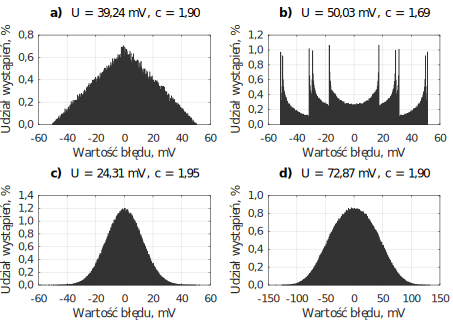
\includegraphics{obrazki/hist_part_S}
\makecaption{fig:symul_partd_hist_S_2_0}{Histogramy błędu \textbf{a)}~statycznego, \textbf{b)}~dynamicznego, \textbf{c)}~losowego, \textbf{d)}~wypadkowego, wielkości wyjściowej $S_{2,0}$ analizowanego w eksperymencie symulacyjnym toru pomiarowego}
\end{center}
\end{figure}

Na podstawie histogramów przedstawionych na rysunkach~\ref{fig:symul_partd_hist_S_2_0} oraz~\ref{fig:symul_partc_hist_T_1_0} zauważyć można, że oszacowane w równaniach od~\eqref{eq:sym_partd_output_unc_roun_S_2_0} do~\eqref{eq:sym_partd_output_unc_dyn_3_S_2_0} oraz od~\eqref{eq:sym_partd_output_unc_roun_T_1_0} do~\eqref{eq:sym_partd_output_unc_dyn_3_T_1_0} parametry sygnałów błędów pokrywają się z tymi uzyskanymi symulacyjnie. Analizując przedstawione na rysunkach parametry błędów losowych zauważyć można, że wpływ błędów zaokrągleń na wypadkowy błąd losowy jest na tyle mały, że błędy te w analizowanej sytuacji mogły zostać pominięte w analizie bez większego wpływu na dokładność jej wyników. Współczynnik $A_{T_{1,0},s} $ określony w równaniu~\eqref{eq:sym_partd_output_as_T_1_0} wskazujący relacje pomiędzy wejściową i wyjściową wariancją błędów statycznych w przypadku wielkości wyjściowej $T_{1,0}$ jest w przybliżeniu równy zero. W rzeczywistości natomiast, ze względu na niewymierność kolejnych współczynników wiersza macierzy transformacji powiązanych z analizowaną wielkością wyjściową, współczynnik ten jest niezerowy. Fakt ten zauważyć można na podstawie rysunku~\ref{fig:symul_partc_hist_T_1_0} gdzie teoretycznie wszystkie realizacje błędu statycznego powinny być zerowe. Omawiana rozbieżność jest jednak bardzo niewielka i nie wopływa zupełnie na uzyskane wyniki obliczeń.

\begin{figure}[htb!]
\begin{center}
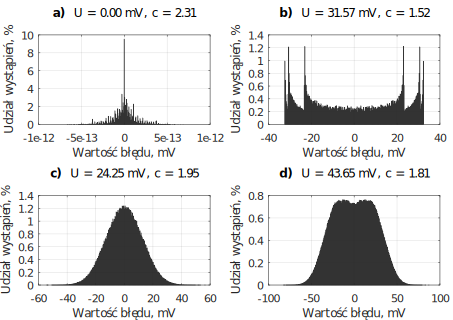
\includegraphics{obrazki/hist_part_T}
\makecaption{fig:symul_partc_hist_T_1_0}{Histogramy błędu \textbf{a)}~statycznego, \textbf{b)}~dynamicznego, \textbf{c)}~losowego, \textbf{d)}~wypadkowego, wielkości wyjściowej $T_{1,0}$ analizowanego w eksperymencie symulacyjnym toru pomiarowego}
\end{center}
\end{figure}

Wobec powyższych informacji wnioskować można, że przeprowadzony eksperyment wykazał poprawność zaproponowanej metody analizy oraz stworzonego na potrzeby pracy modelu błędu. Oszacowana przy użyciu proponowanej metody wartość wariancji dla analizowanych źródeł błędów oraz dla błędów wypadkowych każdorazowo okazywała się zbieżna z wartością uzyskaną metodą symulacyjną. Uzyskane wartości niepewności rozszerzonej wyznaczane z użyciem redukcyjnej arytmetyki interwałowej cechowały się rozbieżnością na poziomie mniejszym niż $3.5\%$, a zatem również uznać można je za poprawne. Eksperyment wykazał możliwość stosowania uproszczenia obliczeń, które wynika bezpośrednio z warunków centralnego twierdzenia granicznego, natomiast stosowanie go dopuszczone jest tylko i wyłącznie w określonych warunkach. Stosowanie założeń centralnego twierdzenia granicznego w przypadkach o niewielkiej liczbie niezależnych źródeł błędów lub w przypadkach istnienia dominującego źródła błędu skutkować będzie przekraczającym $5\%$ błędem oszacowania niepewności rozszerzonej, co w wielu przypadkach może być uznawane za niedopuszczalne.

Zgodnie z założeniami przedstawionymi we wstępie podrozdziału, ostatnią czynnością weryfikującą symulacyjnie poprawność przedstawionych w pracy założeń będzie przeprowadzenie powyższej analizy wykorzystując budżet niepewności zestawiony w tabeli~\ref{tab:sym_partc_params_unc_list}. Jako, że analiza kolejnych fragmentów toru pomiarowego wykazała korelacje pomiędzy wybranymi źródłami błędu, wyznaczenie wariancji wypadkowych sygnałów błędów przeprowadzane będzie zgodnie z zależnością~\eqref{eq:alg_outvar_mat}. Podobnie, jak w przykładach poprzednich, wartości wypadkowej niepewności rozszerzonej zostaną oszacowane na dwa sposoby -- z wykorzystaniem równania~\eqref{eq:alg_outunc_mat} oraz z założeniem zbliżonego do normalnego kształtu rozkładu rozkładu błędu wypadkowego, stosując zależność~\eqref{eq:unc_sum}. Jako, że wyznaczanie parametrów kolejnych składowych sygnałów błędów odbywać się będzie analogicznie, jak miało to miejsce w przykładach opisanych zależnościami od~\eqref{eq:sym_partd_output_var_stat_S_2_0} do~\eqref{eq:sym_partd_output_var_dyn_3_S_2_0} oraz od~\eqref{eq:sym_partd_output_unc_stat_S_2_0} do~\eqref{eq:sym_partd_output_unc_dyn_3_S_2_0}, obliczenia te nie będą przedstawiane. W tabeli~\ref{tab:sym_partd_params_unc_list_S_2_0} zestawiono obliczone parametry wszystkich źródeł błędów wielkości wyjściowej $S_{2,0}$, natomiast parametry wielkości wyjściowej $T_{1,0}$ zestawiono w tabeli~\ref{tab:sym_partd_params_unc_list_T_1_0}.

\begin{table}[htb!]
\begin{center}
\makecaption{tab:sym_partd_params_unc_list_S_2_0}{Budżet niepewności wielkości wyjściowej $S_{2,0}$ analizowanego w eksperymencie symulacyjnym toru pomiarowego, gdzie (a) oznacza przetwornik pomiarowy, (b) oznacza wzmacniacz pomiarowy oraz (c) oznacza przetwornik analogowo-cyfrowy}
\begin{tabular}[c]{| c | c | S[table-format = 2.2] | S[table-format = 3.2] | c | c |} \hline
\textbf{Lp.} & \textbf{Symbol} & \textbf{$U_{95\%}$, mV} & \textbf{$\sigma^{2}$, \micro V} & \textbf{Rozkład} & \textbf{Źródło błędu} \\ \hline
1  & ${rw,z}$     & 2.13  &   0.97  & niestandardowy               & operacje zaokrągleń                        \\ \hline
2  & ${rp,q}$     & 13.26 &  45.78  & normalny                     & proces kwantowania (c)                     \\ \hline
3  & ${rp,1}$     & 11.80 &  36.26  & normalny                     & nieliniowość obiektu (a)                   \\ \hline
4  & ${rp,2}$     & 16.70 &  72.64  & normalny                     & szum wielkości wejściowej                  \\ \hline
5  & ${sp,1}$     & 23.04 &  147.00 & trójkątny                    & dryf temperatury (a)                       \\ \hline
6  & ${sp,2}$     & 16.29 &  73.52  & trójkątny                    & dryf temperatury (b)                       \\ \hline
7  & ${dp,a,1}$   & 12.32 &  76.34  & \multirow{6}{*}{dwumodalny}  & \multirow{3}{*}{transmitancja (a)}         \\ \cline{1-4}
8  & ${dp,a,2}$   & 25.08 &  316.38 &                              &                                            \\ \cline{1-4}
9  & ${dp,a,3}$   & 2.35  &  2.77   &                              &                                            \\ \cline{1-4} \cline{6-6}
10 & ${dp,b,1}$   & 6.07  &  18.52  &                              & \multirow{3}{*}{transmitancja (b)}         \\ \cline{1-4}
11 & ${dp,b,2}$   & 12.35 &  76.70  &                              &                                            \\ \cline{1-4}
12 & ${dp,b,3}$   & 1.16  &  0.67   &                              &                                            \\ \hline
\end{tabular}
\end{center}
\end{table}

W dalszej części rozważań przyjmuje się, że symbolem $\bsigma_{*}$ oznaczono wektory złożone z kolejnych odchyleń standardowych sygnałów błędów wielkości wyjściowych algorytmu, gdzie \enquote{$*$} oznacza symbol analizowanej wielkości wyjściowej. Zgodnie z równaniem \eqref{eq:alg_outvar_mat} wartość wariancji wypadkowego sygnału błędu błędu dla wybranej wielkości wyjściowej opisać można jako:
\begin{equation}
\sigma_{*,\Sigma}^{2} = \bsigma_{*}^{T} \cdot \mathbf{h} \cdot \bsigma_{*} \label{eq:sym_partd_output_varmat_list}
\end{equation}
Z uwagi na fakt, że analizowany algorytm nie wpływa na relacje przetwarzanych sygnałów błędu, macierz korelacji oznaczona symbolem $\mathbf{h}_{d}$ będzie jednakowa dla wszystkich wielkości wyjściowych tego algorytmu i składać się będzie z dwunastu wierszy i kolumn. Na podstawie równania \eqref{eq:sym_partb_stat_corr} korelacja pomiędzy błędami statycznymi spowodowanymi wpływem temperatury na charakterystykę wzmacniacza i przetwornika pomiarowego wyniesie $1$, zatem $r_{d,5,6} = 1$. Dodatkowo współczynniki korelacji kolejnych harmonicznych błędu dynamicznego o tej samej częstotliwości są w przybliżeniu równe jedności, zatem: $r_{d,7,10} = r_{d,8,11} = r_{d,9,12} = 1$. W pozostałych przypadkach współczynniki korelacji będą równe $0$, poza przekątną macierzy gdzie wyniosą one $1$. Wobec powyższych macierz korelacji w omawianym przypadku przyjmuje postać:
\begin{equation}
\mathbf{r}_{d} =
\begin{bmatrix}
1.0 & 0.0 & 0.0 & 0.0 & 0.0 & 0.0 & 0.0 & 0.0 & 0.0 & 0.0 & 0.0 & 0.0 \\
0.0 & 1.0 & 0.0 & 0.0 & 0.0 & 0.0 & 0.0 & 0.0 & 0.0 & 0.0 & 0.0 & 0.0 \\
0.0 & 0.0 & 1.0 & 0.0 & 0.0 & 0.0 & 0.0 & 0.0 & 0.0 & 0.0 & 0.0 & 0.0 \\
0.0 & 0.0 & 0.0 & 1.0 & 0.0 & 0.0 & 0.0 & 0.0 & 0.0 & 0.0 & 0.0 & 0.0 \\
0.0 & 0.0 & 0.0 & 0.0 & 1.0 & 1.0 & 0.0 & 0.0 & 0.0 & 0.0 & 0.0 & 0.0 \\
0.0 & 0.0 & 0.0 & 0.0 & 1.0 & 1.0 & 0.0 & 0.0 & 0.0 & 0.0 & 0.0 & 0.0 \\
0.0 & 0.0 & 0.0 & 0.0 & 0.0 & 0.0 & 1.0 & 0.0 & 0.0 & 1.0 & 0.0 & 0.0 \\
0.0 & 0.0 & 0.0 & 0.0 & 0.0 & 0.0 & 0.0 & 1.0 & 0.0 & 0.0 & 1.0 & 0.0 \\
0.0 & 0.0 & 0.0 & 0.0 & 0.0 & 0.0 & 0.0 & 0.0 & 1.0 & 0.0 & 0.0 & 1.0 \\
0.0 & 0.0 & 0.0 & 0.0 & 0.0 & 0.0 & 1.0 & 0.0 & 0.0 & 1.0 & 0.0 & 0.0 \\
0.0 & 0.0 & 0.0 & 0.0 & 0.0 & 0.0 & 0.0 & 1.0 & 0.0 & 0.0 & 1.0 & 0.0 \\
0.0 & 0.0 & 0.0 & 0.0 & 0.0 & 0.0 & 0.0 & 0.0 & 1.0 & 0.0 & 0.0 & 1.0
\end{bmatrix}
\label{eq:sym_partd_output_coher_list}.
\end{equation}
Na podstawie zależności \eqref{eq:sym_partd_output_varmat_list}, macierzy korelacji danej równaniem \eqref{eq:sym_partd_output_coher_list} po podstawieniu danych z tabeli \ref{tab:sym_partd_params_unc_list_S_2_0} otrzymuje się wartość wariancji wypadkowego sygnału błędu wielkości wyjściowej $S_{2,0}$:
\begin{equation}
\sigma_{S_{2,0},\Sigma}^{2} = \bsigma_{S_{2,0}}^{T} \cdot \mathbf{h} \cdot \bsigma_{S_{2,0}} = \qty{1465.10}{\micro V} \label{eq:sym_partd_output_varmat_S_2_0},
\end{equation}
natomiast po podstawieniu wartości z tabeli \ref{tab:sym_partd_params_unc_list_T_1_0} otrzymuje się wartość wariancji wypadkowego sygnału błędu dla wielkości $T_{1,0}$:
\begin{equation}
\sigma_{T_{1,0},\Sigma}^{2} = \bsigma_{T_{1,0}}^{T} \cdot \mathbf{h} \cdot \bsigma_{T_{1,0}} = \qty{1234.56}{\micro V} \label{eq:sym_partd_output_varmat_T_1_0}.
\end{equation}
Można zauważyć, że wyznaczone w ten sposób wartości są identyczne, jak te wyznaczone w równaniach \eqref{eq:sym_partd_output_var_sum_S_2_0} oraz \eqref{eq:sym_partd_output_var_sum_T_1_0}

\begin{table}[htb!]
\begin{center}
\makecaption{tab:sym_partd_params_unc_list_T_1_0}{Budżet niepewności wielkości wyjściowej $T_{1,0}$ analizowanego w eksperymencie symulacyjnym toru pomiarowego, gdzie (a) oznacza przetwornik pomiarowy, (b) oznacza wzmacniacz pomiarowy oraz (c) oznacza przetwornik analogowo-cyfrowy}
\begin{tabular}[c]{| c | c | S[table-format = 2.2] | S[table-format = 3.2] | c | c |} \hline
\textbf{Lp.} & \textbf{Symbol} & \textbf{$U_{95\%}$, mV} & \textbf{$\sigma^{2}$, \micro V} & \textbf{Rozkład} & \textbf{Źródło błędu} \\ \hline
1  & ${rw,z}$     & 1.81  &  0.70   & niestandardowy               & operacje zaokrągleń                        \\ \hline
2  & ${rp,q}$     & 13.26 &  45.78  & normalny                     & proces kwantowania (c)                     \\ \hline
3  & ${rp,1}$     & 11.80 &  36.26  & normalny                     & nieliniowość obiektu (a)                   \\ \hline
4  & ${rp,2}$     & 16.70 &  72.64  & normalny                     & szum wielkości wejściowej                  \\ \hline
5  & ${sp,1}$     & 0.00  &  0.00   & trójkątny                    & dryf temperatury (a)                       \\ \hline
6  & ${sp,2}$     & 0.00  &  0.00   & trójkątny                    & dryf temperatury (b)                       \\ \hline
7  & ${dp,a,1}$   & 0.06  &  0.00   & \multirow{6}{*}{dwumodalny}  & \multirow{3}{*}{transmitancja (a)}         \\ \cline{1-4}
8  & ${dp,a,2}$   & 3.77  &  7.13   &                              &                                            \\ \cline{1-4}
9  & ${dp,a,3}$   & 19.16 &  184.65 &                              &                                            \\ \cline{1-4} \cline{6-6}
10 & ${dp,b,1}$   & 0.03  &  0.00   &                              & \multirow{3}{*}{transmitancja (b)}         \\ \cline{1-4}
11 & ${dp,b,2}$   & 1.85  &  1.73   &                              &                                            \\ \cline{1-4}
12 & ${dp,b,3}$   & 9.44  &  44.82  &                              &                                            \\ \hline
\end{tabular}
\end{center}
\end{table}

asd

\section{Podsumowanie przeprowadzonego eksperymentu}

TODO
